\documentclass{article}

\def\npart {II}
\def\nyear {2017}
\def\nterm {Michaelmas}
\def\nlecturer{Dr C. Brookes}
\def\ncourse{Galois Theory}
\usepackage{imakeidx}
\ifx \nauthor\undefined
  \def\nauthor{Bhavik Mehta}
\else
\fi

\author{Based on lectures by \nlecturer \\\small Notes taken by \nauthor}
\date{\nterm\ \nyear}
\title{Part \npart\ -- \ncourse}

\usepackage[utf8]{inputenc}
\usepackage{amsmath}
\usepackage{amsthm}
\usepackage{amssymb}
\usepackage{enumerate}
\usepackage{mathtools}
\usepackage{graphicx}
\usepackage[dvipsnames]{xcolor}
\usepackage{tikz}
\usepackage{wrapfig}
\usepackage{centernot}
\usepackage{float}
\usepackage{braket}
\usepackage[hypcap=true]{caption}
\usepackage{enumitem}
\usepackage[colorlinks=true, linkcolor=mblue]{hyperref}
\usepackage[nameinlink,noabbrev]{cleveref}
\usepackage{nameref}
\usepackage[margin=1.5in]{geometry}

% Theorems
\theoremstyle{definition}
\newtheorem*{aim}{Aim}
\newtheorem*{axiom}{Axiom}
\newtheorem*{claim}{Claim}
\newtheorem*{cor}{Corollary}
\newtheorem*{conjecture}{Conjecture}
\newtheorem*{defi}{Definition}
\newtheorem*{eg}{Example}
\newtheorem*{ex}{Exercise}
\newtheorem*{fact}{Fact}
\newtheorem*{law}{Law}
\newtheorem*{lemma}{Lemma}
\newtheorem*{notation}{Notation}
\newtheorem*{prop}{Proposition}
\newtheorem*{question}{Question}
\newtheorem*{rrule}{Rule}
\newtheorem*{thm}{Theorem}
\newtheorem*{assumption}{Assumption}

\newtheorem*{remark}{Remark}
\newtheorem*{warning}{Warning}
\newtheorem*{exercise}{Exercise}

% \newcommand{\nthmautorefname}{Theorem}

\newtheorem{nthm}{Theorem}[section]
\newtheorem{nlemma}[nthm]{Lemma}
\newtheorem{nprop}[nthm]{Proposition}
\newtheorem{ncor}[nthm]{Corollary}
\newtheorem{ndef}[nthm]{Definition}

% Special sets
\newcommand{\C}{\mathbb{C}}
\newcommand{\N}{\mathbb{N}}
\newcommand{\Q}{\mathbb{Q}}
\newcommand{\R}{\mathbb{R}}
\newcommand{\Z}{\mathbb{Z}}

\newcommand{\abs}[1]{\left\lvert #1\right\rvert}
\newcommand{\norm}[1]{\left\lVert #1\right\rVert}
\renewcommand{\vec}[1]{\boldsymbol{\mathbf{#1}}}

\let\Im\relax
\let\Re\relax

\DeclareMathOperator{\Im}{Im}
\DeclareMathOperator{\Re}{Re}
\DeclareMathOperator{\id}{id}

\definecolor{mblue}{rgb}{0., 0.05, 0.6}

\makeindex[intoc]

% preamble
\setcounter{section}{-1}
\usepackage{tkz-euclide}
\usepackage{xfrac}
\usepackage{stmaryrd}
\SetSymbolFont{stmry}{bold}{U}{stmry}{m}{n}
\usetkzobj{all}
\usetikzlibrary{cd, backgrounds}

\DeclareMathOperator{\Aut}{Aut}
\DeclareMathOperator{\chara}{char}
\DeclareMathOperator{\Tr}{Tr}
\DeclareMathOperator{\Gal}{Gal}
\DeclareMathOperator{\Ker}{Ker}

\newtheorem{nexample}[nthm]{Example}
\newtheorem{nremark}[nthm]{Remark}
\newcommand{\F}{\mathbb{F}}

\newtheorem{manualinner}{}
\newenvironment{manual}[1]{%
    \renewcommand\themanualinner{#1}%
    \manualinner
}{\endmanualinner}
% and here we go!


\begin{document}
\maketitle

% lecture 1

\clearpage
\section{Introduction}

\subsection{Course overview}










% Galois' papers have been studied by Peter Neumann:
% The math writings of Evariste Galois, European Math Soc
% Different books: I. Steward Galois Theory, (something) and Hall
% contains a historcal introduction and covers almost all the syllabus.
% Artin Galois Theory
% Van der Waerden Modern Algebra (covers a lot more than Galois theory)
% Lang Algebra (late editions are preferred, covers a lot of algebra)
% Kaplansky Fields and Rings


\clearpage
\section{Field Extensions}\label{sec:1}









\begin{nthm}[Tower law]\index{tower law}\label{thm:towerLaw}
    Suppose $K \leq L \leq M$ are field extensions. Then $\abs{M:K}$ = $\abs{M:L}\abs{L:K}$.
\end{nthm}
\begin{proof}
    Assume that $\abs{M:L} < \infty$, and $\abs{L:K} < \infty$.
    Take an $L$-basis of $M$, given by $\Set{f_1, \dotsc, f_b}$, and a $K$-basis of $L$ given by $\Set{e_1, \dotsc, e_a}$.
    Take $m \in M$, so $m = \sum_{i=1}^b \mu_i f_i$ for some $\mu_i \in L$.
    Similarly, $\mu_i = \sum_{j=1}^a \lambda_{ij} e_j$ for some $\lambda_{ij} \in K$, so

    \begin{equation*}
        m = \sum_{i=1}^b \sum_{j=1}^a \lambda_{ij} e_j f_i
    \end{equation*}
    Thus $\Set{e_j f_i | 1 \leq j \leq a, 1 \leq i \leq b}$ span $M$.

    Linear independence:
    It's enough to show that if $0 = m = \sum \sum \lambda_{ij} e_j f_i$ then $\lambda_{ij}$ are all zero.
    However if $m = 0$ the linear independence of $f_i$ forces each $\mu_i = 0$.
    Then the linear indepedence of $e_j$ forces $\lambda_{ij}$ all to be zero, as required.
\end{proof}









\subsection{Motivatory Example}\label{sec:motivEg}







% new lec (2)



























\subsection{Review of GRM}



\begin{nlemma}\label{lem:1.5}
    Let $K \leq L$ be a finite field extension. Then $L$ is algebraic over $K$.
\end{nlemma}
\begin{proof}
    Let $\abs{L:K}=n$, and take $\alpha \in L$. Consider $1, \alpha, \alpha^2, \dotsc, \alpha^n$, which must be linearly dependent in the $n$-dimensional $K$--vector space $L$.
    So, $\sum_{i=0}^n \lambda_i \alpha^i = 0$ for some $\lambda \in K$ not all zero, and hence $\alpha$ is a root of $f(t) = \sum_{i=0}^n \lambda_i t^i$, so $\alpha$ is algebraic over $K$.
    $\alpha$ was arbitrary, so $L$ is algebraic over $K$.
\end{proof}



\begin{nlemma}\label{lem:1.7}
    Suppose $K \leq L$ is a field extension, $\alpha \in L$ and $\alpha$ is algebraic over $K$.
    Then the minimal polynomial $f_\alpha(t)$ of $\alpha$ over $K$ is irreducible in $K[t]$ and $I_\alpha$ is a prime ideal.
\end{nlemma}
\begin{proof}
    Suppose $f_\alpha(t) = p(t) q(t)$. We aim to show $p(t)$ or $q(t)$ is a unit in $K[t]$.
    But $0 = f_\alpha(\alpha) = p(\alpha) q(\alpha)$, so $p(\alpha) = 0$ or $q(\alpha) = 0$, without loss of generality take $p(\alpha) = 0$, thus $p(t) \in I_\alpha$.

    But $I_\alpha=(f_\alpha(t))$, so $p(t) = f_\alpha(t) r(t)$, giving $f_\alpha(t) = f_\alpha(t) r(t) q(t)$ and so $r(t) q(t) = 1$ in $K[t]$, and $q(t)$ is a unit, as required.
    Recall from GRM that irreducible elements of $K[t]$ are prime and hence generate prime ideals of $K[t]$. So $I_\alpha$ is a prime ideal.
\end{proof}

% new lec (3)

\begin{nthm}\label{thm:1.9}
    Suppose $K \leq L$ is a field extension and $\alpha \in L$ is algebraic over $K$.  Then
    \begin{enumerate}[label=(\roman*)]
        \item  $K(\alpha) = K[\alpha]$
        \item $\abs{K(\alpha) : K} = \deg f_\alpha(t)$ where $f_\alpha(t)$ is the minimal polynomial of $\alpha$ over $K$.
    \end{enumerate}
\end{nthm}
\begin{proof}\leavevmode
    \begin{enumerate}[label=(\roman*)]
        \item Clearly $K[\alpha] \leq K(\alpha)$. We aim to show that any non-zero element $\beta$ of $K[\alpha]$ is a unit, so $K[\alpha]$ is a field.

            By definition of $K[\alpha]$, we have $\beta = g(\alpha)$ for some $g(t) \in K[t]$.
            Since $\beta = g(\alpha) \neq 0$, $g(t) \notin I_\alpha = (f_\alpha(t))$.
            Thus $f_\alpha(t) \nmid g(t)$.

            From \cref{lem:1.7}, $f_\alpha(t)$ is irreducible and $K[t]$ is a PID, we know $\exists r(t), s(t) \in K[t]$ with
            \begin{equation*}r(t) f_\alpha(t) + s(t) g(t) = 1 \in K[t].\end{equation*}
            Hence $s(\alpha) g(\alpha) = 1$ in $K[\alpha]$, and so $\beta = g(\alpha)$ is a unit, as required.
        \item Let $n = \deg f_\alpha(t)$ We'll show that $T = \set{1, \alpha, \alpha^2, \dotsc, \alpha^{n-1}}$ is a $K$--vector space basis of $K[\alpha]$.

            Spanning: If $f_\alpha(t) = t^n + a_{n-1} t^{n-1} + \dots + a_0$ with $a_i \in K$, then $\alpha^n = -a_{n-1} \alpha^{n-1} - \dots - a_0$.
            This implies $\alpha^n$ is a linear combination of $\set{1, \alpha, \alpha^2, \dotsc, \alpha^{n-1}}$, and an easy induction shows that $\alpha^m$ for $m \geq n$ is likewise a linear combination of $\set{1, \alpha, \alpha^2, \dotsc, \alpha^{n-1}}$, so we have spanning.

            Linear independence: Suppose $\lambda_{n-1} \alpha^{n-1} + \dotsc + \lambda_0 = 0$.
            Let $g(t) = \lambda_{n-1} t^{n-1} + \dotsc + \lambda_0$.  Since $g(\alpha) = 0$, we have $g(t) \in I_\alpha = (f_\alpha(t)).$  So $g(t) = 0$ or $f_\alpha(t) \mid g(t)$.
            The latter is not possible since $\deg f_\alpha(t) > \deg g_\alpha(t)$ so $g(t) = 0$ in $K[t]$ and all the $\lambda_i$'s are zero. \qedhere
    \end{enumerate}
\end{proof}
\begin{ncor}\label{cor:1.10}
    If $K \leq L$ is a field extension and $\alpha \in L$, then $\alpha$ is algebraic over $K$ if and only if $K \leq K(\alpha)$ is finite.
\end{ncor}
\begin{proof} \leavevmode
    \begin{itemize}
        \item[($\Rightarrow$)] By \cref{thm:1.9}, $\abs{K(\alpha):K} = \deg f_\alpha(t) \leq \infty$.
        \item [($\Leftarrow$)] \Cref{lem:1.5}
    \end{itemize}
\end{proof}
\begin{ncor}\label{cor:1.11}
    Let $K \leq L$ be a field extension with $\abs{L:K} = n$. Let $\alpha \in L$, then $\deg f_\alpha(t) \mid n$.
\end{ncor}
\begin{proof}
    Use the \nameref{thm:towerLaw} on $K \leq K(\alpha) \leq L$.
    We deduce that $\abs{K(\alpha):K}$ divides $\abs{L:K}$.
    \Cref{thm:1.9}(ii) gives $\deg f_\alpha(t) = \abs{K(\alpha) : K}$.
\end{proof}
\subsection{Digression on (Non-)Constructibility}















\begin{nlemma}\label{lem:1.13}
    $x_i, y_i$ are both roots in $K_i$ of quadratic polynomials in $K_{i-1}[t]$.
\end{nlemma}
\begin{proof}
    There are three cases for $\vec{r_i}$: line meets line, line meets circle, circle meets circle. We do the second case only here.
    \begin{center}
        \begin{tikzpicture}[scale=1]
            \tkzDefPoint[label=below:$A$](-0.5,1){A}
            \tkzDefPoint[label=below:$B$](3,2){B}
            \tkzDefPoint[label=below:$C$](0,0){C}

            \tkzDrawCircle[R, very thin](C, 2.5cm)
            \tkzDrawSegment[very thin, add=3cm and 1cm](A, B)

            \tkzInterLC[R](A,B)(C,2.5cm) \tkzGetPoints{X}{Y}
            \tkzLabelPoints[above left](X)
            \tkzLabelPoints[above](Y)

            \tkzDrawPoints[fill=black](A,B,C,X,Y)
            % \draw (0, 0) circle [radius=2];
            % \draw (-3, 0) -- (3, 2);
        \end{tikzpicture}
    \end{center}
    The line is defined by two points $A = (p, q)$ and $B = (r, s)$ while the circle is defined with a centre $C = (t, u)$ and radius $w$.
    Then, points $X$ and $Y$ satisfy the equation of the line $\frac{x-p}{r-p} = \frac{y-q}{s-q}$, and the equation of the circle $(x-t)^2 + (y-u)^2 = w^2$.
    Solving these together gives coordinates of $X$ and $Y$ satisfying quadratic polynomials over $K_{i-1}$.
    The other two cases are left as an exercise for the reader.
\end{proof}
% new lec (4)

\begin{nthm}\label{thm:1.14}
    If $\vec{r} = (x, y)$ is constructible from a set $P_0$ of points in $\R^2$ and if $K_0$ is the subfield of $\R$ generated by $\Q$ and the coordinates of the points in $P_0$, then the degrees $\abs{K_0(x) : K_0}$ and $\abs{K_0(y):K_0}$ are powers of two.
\end{nthm}
\begin{proof}
    Continue with the previous notation of $K_i = K_{i-1}(x_i, y_i)$. By the \nameref{thm:towerLaw},
    \begin{equation*}
        \abs{K_i : K_{i-1}} = \abs{K_{i-1} (x, y): K_{i-1}(x)} \abs{K_{i-1}(x) : K_{i-1}}
    \end{equation*}
    But \cref{lem:1.13} tells us that $\abs{K_{i-1}(x):K_{i-1}}$ must be $1$ or $2$ depending on whether the quadratic polynomial arising in the lemma is reducible or not, using \cref{thm:1.9}(ii). Similarly, $\abs{K_{i-1}(x, y):K_{i-1}(x)}$ is 1 or 2.

    So $\abs{K_i: K_{i-1}} = 1, 2 \ \text{or} \ 4$, (but in fact $4$ cannot happen), hence by the \nameref{thm:towerLaw}, $\abs{K_n:K_0} = \abs{K_n:K_{n-1}} \abs{K_{n-1} : K_{n-2}} \dots \abs{K_1:K_0}$ is a power of two.

    If $r = (x, y)$ is constructible from $P_0$, then
    \begin{align*}
        x, y \in K_n \quad \text{and} \quad K_0 &\leq K_0(x) \leq K_n \\
        K_0 &\leq K_0(y) \leq K_n
    \end{align*}
    and the Tower Law again gives that $|K_0(x):K_0|$ and $|K_0(y):K_0|$ are also powers of $2$.
\end{proof}


\begin{nthm}\label{thm:1.15}
    Let $f(t)$ be a primitive integral polynomial.  Then $f(t)$ is irreducible in $\Q[t]$ if and only if it is irreducible in $\Z[t]$.
\end{nthm}
\begin{proof}
    A special case of Gauss' lemma from GRM.
\end{proof}
\begin{nthm}[Eisenstein's criterion]\index{Eisenstein's criterion}\label{thm:1.16}
    Let $f(t) = a_n t^n + a_{n-1} t^{n-1} + \dots + a_0 \in \Z[t]$.
    Suppose there is a prime $p$ such that
    \begin{enumerate}[label=(\roman*)]
        \item $p \nmid a_n$
        \item $p \mid a_{n-1}, \, p \mid a_{n-2}, \dotsc, p \mid a_0$
        \item $p^2 \nmid a_0$
    \end{enumerate}
    Then $f(t)$ is irreducible in $\Z[t]$
\end{nthm}
\begin{proof}
    Recall from GRM.
\end{proof}











% back to non-constructibility
\begin{nthm}\label{thm:1.17}
    The cube cannot be duplicated by ruler and compasses.
\end{nthm}
\begin{proof}
    The problem amounts to whether given a unit distance, one can construct points distance $\alpha$ apart, where $\alpha$ satisfies $t^3 - 2 = 0$.
    Starting with points $P_0 = \{(0, 0), (1, 0)\}$ can we produce $(\alpha, 0)$?

    No. If we could, \cref{thm:1.14} would say $\abs{\Q(\alpha):\Q}$ is a power of 2. But $\abs{\Q(\alpha): \Q} = 3$ since $\abs{\Q(\alpha):\Q} = \deg f_\alpha(t)$ where $f_\alpha(t)$ is the minimal polynomial of $\alpha$ over $\Q$. $\alpha$ satisfies $t^3 - 2$, which is irreducible over $\Z$ by \nameref{thm:1.16} hence irreducible over $\Q$. So $t^3 - 2$ is the minimal polynomial $f_\alpha(t)$.
\end{proof}
\begin{nthm}\label{thm:1.18}
    The circle cannot be squared using ruler and compasses.
\end{nthm}
\begin{proof}
    Starting with $(0, 0)$ and $(1, 0)$, we must construct $(\sqrt{\pi}, 0)$ so that we have a square of side length $\sqrt{\pi}$ and hence area $\pi$.
    But $\pi$ and hence $\sqrt{\pi}$ is transcendental over $\Q$ (Lindemann - not proved here).
    \Cref{thm:1.14} tells us we can't do this construction.
\end{proof}
\subsection{Return to theory development}
\begin{nlemma}\label{lem:1.19}
    Let $K \leq L$ be a field extension. Then
    \begin{enumerate}[label=(\roman*)]
        \item $\alpha_1, \dotsc, \alpha_n \in L$ are algebraic over $K$ if and only if $K \leq K(\alpha_1, \dotsc, \alpha_n)$ is a finite field extension.
        \item If $K \leq M \leq L$ such that $K \leq M$ is finite, then there exist $\alpha_1, \dotsc, \alpha_n \in L$ such that $K(\alpha_1, \dotsc, \alpha_n) = M$.
    \end{enumerate}
\end{nlemma}
\begin{proof} \leavevmode
    \begin{enumerate}[label=(\roman*)]
        \item By \cref{cor:1.10}, $\alpha$ is algebraic over $K$ if and only if $K \leq K[\alpha]$ is a finite field extension.
            $\alpha_i$ is algebraic over $K$ and hence algebraic over $K(\alpha_1, \dotsc, \alpha_{i-1})$ and so
            \begin{equation*}\abs{K(\alpha_1, \dotsc, \alpha_i):K(\alpha_1, \dotsc, \alpha_{i-1})} < \infty.\end{equation*}
            By the \nameref{thm:towerLaw} applied to
            \begin{equation*}K \leq K(\alpha_1) \leq K(\alpha_1, \alpha_2) \leq \dots \leq K(\alpha_1, \dotsc, \alpha_n),\end{equation*} we get $\abs{K(\alpha_1, \dotsc, \alpha_n):K} < \infty$.

            Conversely, consider $K \leq K(\alpha_i) \leq K(\alpha_1, \dotsc, \alpha_n)$.
            Then the tower law says that if $\abs{K(\alpha_1, \dotsc, \alpha_n): K} < \infty$ then $\abs{K(\alpha_i):K} < \infty$ and by \cref{cor:1.10}, $\alpha_i$ is algebraic over $K$.

        \item If $\abs{M:K} = n$ then $M$ is an $n$-dimensional $K$-vector space, so there exists a $K$-basis $\alpha_1, \dotsc, \alpha_n$ over $M$.
            Then $K(\alpha_1, \dotsc, \alpha_n) \leq M$.
            However, any element of $M$ is a $K$-linear combination of $\alpha_1, \dotsc, \alpha_n$ and so lies in $K(\alpha_1, \dotsc, \alpha_n)$, so $M = K(\alpha_1, \dotsc, \alpha_n)$. \qedhere
    \end{enumerate}
\end{proof}
% new lec (5)


\begin{nlemma}\label{lem:1.21}
    Suppose $K \leq L$, $K \leq L'$ are field extensions. Then
    \begin{enumerate}[label=(\roman*)]
        \item Any $K$-homomorphism $\phi:L \to L'$ is injective and $K \leq \phi(L)$ is a field extension.
        \item If $|L:K| = |L':K| < \infty$ then any $K$-homomorphism $\phi:L \to L'$ is a $K$-isomorphism.
    \end{enumerate}
\end{nlemma}
\begin{proof} \leavevmode
    \begin{enumerate}[label=(\roman*)]
        \item $L$ is a field and $\ker \phi$ is an ideal of $L$.

            Note $1 \mapsto 1$ and so $\ker \phi$ can't be the whole of $L$, hence $\ker \phi = \{0\}$.
            So $\phi(L)$ is a field and $K \leq \phi(L)$ is a field extension.
        \item $\phi$ is an injective $K$-linear map, so $|\phi(L):K| = |L:K|$.
            In general, $|\phi(L):K| \leq |L':K|$, but since $|L:K| = |L':K|$ by assumption, we have $|\phi(L):K| = |L':K|$, hence $\phi(L) = L'$ and $\phi$ is a $K$-isomorphism $L \to L'$.
            (If $L' = L$ then $\phi$ would be a $K$-automorphism also.) \qedhere
    \end{enumerate}
\end{proof}
% \begin{notation}
%     If $K \leq L$ is a \hyperlink{def:fieldExt}{field extension} and $f(t) \in K[t]$, we denote the set of roots of $f$ in $L$ by $\Root_f(L)$.
% \end{notation}




\begin{nthm}[Existence of splitting fields]\index{splitting field!existence}\label{thm:1.23}
    Let $K$ be a field and $f(t) \in K[t]$. Then there exists a splitting field for $f$ over $K$.
\end{nthm}
\begin{proof}
    If $\deg f = 0$ then $K$ is the splitting field for $f$ over $K$.

    Suppose $\deg f > 0$ and pick an irreducible factor $g(t)$ of $f(t)$ in $K[t]$, noting that $K \leq K[t] / (g(t))$ is a field extension.

    Take
    \begin{equation*}\alpha_1 = t + (g(t)) \in K[t]/(g(t)),\end{equation*}
    then $K[t]/(g(t)) = K(\alpha_1)$ and $g(\alpha_1) = 0$ in $K(\alpha_1)$.
    Therefore $f(\alpha_1) = 0$ in $K(\alpha_1)$ and we can write $f(t) = (t-\alpha_1) h(t)$ in $K(\alpha_1)[t]$.

    Repeat, noting that $\deg h(t) < \deg f(t)$ and so we get
    \begin{equation*}f(t) = a(t - \alpha_1)(t - \alpha_2) \dotsm (t-\alpha_n)\end{equation*}
    where $a$ is a constant in $K$.
    Thus, we have a factorisation of $f(t)$ in $K(\alpha_1, \dotsc, \alpha_n)[t]$, and so $K(\alpha_1, \dotsc, \alpha_n)$ is a splitting field for $f$ over $K$.
\end{proof}
\begin{nthm}[Uniqueness of splitting fields]\index{splitting field!uniqueness}\label{thm:1.24}
    If $K$ is a field and $f(t) \in K[t]$, then the splitting field for $f$ over $K$ is unique up to $K$-isomorphism, that is, if there are two such splitting fields $L$ and $L'$, there is a $K$-isomorphism $\phi: L \to L'$.
\end{nthm}
% new lec (6)

% need to make sure this makes sense
\begin{proof}
    Suppose $L$ and $L'$ are splitting fields for $f(t) \in K[t]$ over $K$. We need to show that there is a $K$-isomorphism $L \to L'$.

    Suppose $K \leq M \leq L$ and there exist $M'$ with $K \leq M' \leq L'$ and a $K$-isomorphism $\psi: M \to M'$.
    Clearly some $M$ exists (we can take $M=K$), so we pick $M$ so that $\abs{M:K}$ is maximal among all such $M, M', \psi$.

    We must show $M=L$ and $M' = L'$. Note that if $M = L$ then $f(t)$ splits over $M$:
    \begin{equation*}
        f(t) = a(t - \alpha_1) \dotsm (t - \alpha_n) \in M[t]
    \end{equation*}
    Apply $\psi$, we get an induced map $M[t] \to M'[t]$.
    \begin{equation*}
        f(t) = \psi(f(t)) = \psi(a) (t - \psi(\alpha_1)) \dotsm (t - \psi(\alpha_n))
    \end{equation*}
    Thus $f(t)$ splits over $\psi(M) = M'$. But $L'$ is a splitting field and $M' \leq L'$, so $M'=L'$.

    So, suppose $M\neq L$ and we'll get a contradiction of maximality of $M$.
    Since $M \neq L$, there is a root $\alpha$ of $f(t)$ in $L$ which isn't in $M$.
    Factorise $f(t) = g(t) h(t)$ in $M[t]$ so that $g(t)$ is irreducible in $M[t]$ while $g(\alpha) = 0$ in $L$.
    Then there exists a $K$-homomorphism $M[t]/(g(t)) \to L$ given by $t + (g(t)) \mapsto \alpha$ which has image $M(\alpha)$.

    The $K$-isomorphism $M[t] \to M'[t]$ induced by $\psi$ maps $g(t) \in M[t]$ to $\gamma(t) \in M'[t]$.
    $f(t) = g(t) h(t)$ in $M[t]$ yields $f(t) = \gamma(t) \delta(t)$ in $M'[t]$.

    We have a field extension $M' \leq M'[t]/(\gamma(t))$ and there exists a $M'$-homomorphism $M'[t]/(\gamma(t)) \to L'$ given by $t + (\gamma(t))$ by picking a root $\alpha'$ of $\gamma(t)$ in $L'$.
    However $\gamma(t) \mid f(t)$ in $M'[t]$ and hence in $L'[t]$ and so $\alpha'$ is also a root of $f(t)$ in $L'$.
    The $M'$-homomorphism gives a $K$-isomorphism
    \begin{equation*}
        M'[t] / (\gamma(t)) \to M'(\alpha')
    \end{equation*}
    and so we have a $K$-isomorphism $M(\alpha) \to M'(\alpha')$. This contradicts the maximality of $M$, since $M \lneqq M(\alpha)$.
\end{proof}

\begin{nthm}\label{thm:1.26}
    Let $K \leq L$ be a finite field extension. Then $K \leq L$ is normal $\iff$ $L$ is the splitting field for some $f(t) \in K[t]$.
\end{nthm}
\begin{proof}
    Later.
\end{proof}

\begin{nthm}\label{thm:1.28}
    Let $G$ be a finite subgroup of the multiplicative group of a field $K$. Then $G$ is cyclic. In particular, the multiplicative group of a finite field is cyclic.
\end{nthm}
\begin{proof}
    Let $\abs{G} = n$. By the structure theorem of finite abelian groups from GRM,
    \begin{equation*}
        G \cong C_{q_1^{m_1}} \times C_{q_2^{m_2}} \times \dotsm \times C_{q_r^{m_r}}
    \end{equation*}
    with $q_i$ prime, not necessarily distinct.
    However if $q = q_i = q_j$ for some $i \neq j$, there are at least $q^2$ distinct solutions of $t^q - 1 = 0$ in $K$ (since $C_q \times C_q \cong$ subgroup of $G$).
    But in a field (or even an integral domain), a polynomial of degree $q$ has at most $q$ roots, a contradiction.
    So all the $q_i$ are distinct and hence $G$ is cyclic, generated by $(g_1, \dotsc, g_r)$ where $g_i$ generates $C_{q_i^{m_i}}$ using the Chinese Remainder Theorem.
\end{proof}
\clearpage
\section{Separable, normal and Galois extensions}

% new lec (7)


\begin{nlemma}\label{lem:2.3}
    Let $K$ be a field and $f(t), g(t) \in K[t]$. Then:
    \begin{enumerate}[label=(\alph*)]
        \item $D(f(t) g(t)) = f'(t) g(t) + f(t) g'(t)$ (Leibniz' rule)
        \item Assume $f(t) \neq 0$. Then $f(t)$ has a repeated root in a splitting field $L$ if and only if $f(t)$ and $f'(t)$ have a common irreducible factor in $K[t]$.
    \end{enumerate}
\end{nlemma}
\begin{proof}
    \leavevmode
    \begin{enumerate}[label=(\alph*)]
        \item $D$ is a $K$-linear map and so we only need to check for $f(t) = t^n$, $g(t) = t^m$. Left as an exercise.
        \item Let $\alpha$ be a repeated root in a splitting field $L$, then
            \begin{align*}
                f(t) &= (t-\alpha)^2 g(t) \in L[t] \\
                f'(t) &= (t-\alpha)^2 g'(t) + 2(t-\alpha) g(t)
            \end{align*}
            and so $f'(\alpha) = 0$.
            Therefore the minimal polynomial $f_\alpha(t)$ of $\alpha$ in $K[t]$ divides both $f(t)$ and $f'(t)$ and thus $f_\alpha(t)$ is a common irreducible factor of $f(t)$ and $f'(t)$.


            Conversely, let $h(t)$ be a common irreducible factor of $f(t)$ and $f'(t)$ in $K[t]$.
            Pick a root $\alpha$ in $L$ of $h(t)$.

            So $f(\alpha) = 0 = f'(\alpha)$, thus $f(t) = (t-a) g(t)$ in $L[t]$, and $f'(t) = (t-a) g'(t) + g(t)$.
            Since $f'(\alpha)  = 0$ we have $(t-a) \mid f'(t)$. and so $(t-a) \mid g(t)$. Hence $(t-a)^2 \mid f(t)$ and we have a repeated root. \qedhere
    \end{enumerate}
\end{proof}
\begin{ncor}\label{cor:2.4}
    If $K$ is a field and $f(t) \in K[t]$ is irreducible:
    \begin{enumerate}[label=(\roman*)]
        \item If the characteristic of $K$ is 0, then $f(t)$ is separable over $K$.
        \item If the characteristic of $K$ is $p>0$, then $f(t)$ is not separable if and only if $f(t) \in K[t^p]$.
    \end{enumerate}
\end{ncor}
\begin{proof}
    By \cref{lem:2.3}, $f(t)$ is not separable over $K$ if and only if $f(t)$ and $f'(t)$ have a common irreducible factor.
    Since we're assuming $f(t)$ is irreducible, this is equivalent to saying $f'(t) = 0$.

    \begin{align*}
        f(t) &= a_n t^n + a_{n-1} t^{n-1} + \dotsb + a_0 \\
        f'(t) &= n a_n t^{n-1} + \dotsb + a_1
    \end{align*}
    Thus $f'(t) = 0 \iff i a_i = 0$ for all $i > 0$.

    \begin{enumerate}[label=(\roman*)]
        \item If $\chara K = 0$ then $f'(t) \neq 0$ for any non-constant polynomial, so $f(t)$ is separable over $K$.
        \item If $\chara K = p > 0$ then if $f'(t) = 0$ we have $i a_i = 0$ for all $i > 0$, so $f(t)$ is not separable $\iff f(t) \in K[t^p]$. \qedhere
    \end{enumerate}
\end{proof}



\begin{nlemma}\label{lem:2.6}
    Let $M = K(\alpha)$, where $\alpha$ is algebraic over $K$ and let $f_\alpha(t)$ be the minimal polynomial of $\alpha$ over $K$.

    Then, for any field extension $K \leq L$, the number of $K$-homomorphisms of $M$ to $L$ is equal to the number of distinct roots of $f_\alpha(t)$ in $L$.
    Thus this number is $\leq \deg f_\alpha(t) = \abs{K(\alpha):K} = \abs{M:K}$.

    \begin{center}
        \begin{tikzpicture}[scale=0.8]
            \node (K) at ( 0,-2)    {$K$};
            \node (L) at ( 2, 2)    {$L$};
            \node (M) at (-2, 0)    {$M = K(\alpha)$};

            \draw (M) -- (K) -- (L);
        \end{tikzpicture}
    \end{center}
\end{nlemma}
\begin{proof}
    We saw in \cref{lem:1.21} that any $K$-homomorphism $M \to L$ is injective, and we have
    \begin{equation*}
        K(\alpha) \cong \frac{K[t]}{(f_\alpha(t))}.
    \end{equation*}
    For any root $\beta$ of $f_\alpha(t)$ in $L$ we can define a $K$-homomorphism
    \begin{align*}
        \frac{K[t]}{(f_\alpha(t))} &\to L \\
        t + (f_\alpha(t)) &\mapsto \beta
    \end{align*}
    Thus we get a $K$-homomorphism $M \to L$.

    Conversely, for any $K$-homomorphism $\phi:M \to L$ the image $\phi(\alpha)$ must satisfy
    \begin{equation*}f_\alpha(\phi(\alpha)) = 0.\end{equation*}
    These processes are inverse to each other, giving a 1-1 correspondence
    \begin{equation*}
        \{K \text{ homomorphisms } M \to L\} \longleftrightarrow \{\text{roots of } f_\alpha(t) \in L\}. \qedhere
    \end{equation*}
\end{proof}
% new lec (8)


\begin{ncor}\label{cor:2.7}
    The number of $K$-homomorphisms $K(\alpha) \to L = \deg f_\alpha(t) \iff L$ is large enough, in particular $L$ contains a splitting field for $f_\alpha(t)$ and $\alpha$ is separable over $K$.
\end{ncor}
\begin{proof}
    Immediate from \cref{lem:2.6}.
\end{proof}
\begin{nlemma}\label{lem:2.8}
    Let $K \leq M$ be a field extension and $M_1 = M(\alpha_1)$ (where $\alpha_1$ is algebraic over $M$).
    Let $f(t)$ be the minimal polynomial of $\alpha_1$ over $M$ and let $K \leq L$.
    Let $\phi: M \to L$ be a $K$-homomorphism. Then there is a correspondence
    \begin{equation*}
        \{\text{Extensions } \phi_1:M_1 \to L \text{ of } \phi\} \longleftrightarrow \{\text{roots of} \ \phi(f(t)) \in L\}.
    \end{equation*}
    \begin{center}
        \begin{tikzpicture}
            \node (K)  at ( 0,-2)    {$K$};
            \node (M)  at (-1, -0.5)    {$M$};
            \node (M1) at (-2, 1)    {$M_1$};
            \node (L)  at ( 2, 2)    {$L$};

            \draw (M1) -- (M) -- (K) -- (L);
        \end{tikzpicture}
    \end{center}
\end{nlemma}

\begin{proof}
    $f(t)$ is irreducible in $M[t]$, so $\phi(f(t))$ is irreducible in $\phi(M)[t]$.
    Any extension $\phi_1: M \to L$ of $\phi$ produces a root $\phi_1(\alpha_1)$ of $\phi(f(t))$.

    Conversely, given a root $\gamma$ of $\phi(f(t))$ in $L$,
    \begin{equation*}
        M_1 = M(\alpha_1) \cong \frac{M[t]}{(f(t))} \cong \frac{\phi(M)[t]}{(\phi(f(t)))} \cong \phi(M)(\phi) \leq L.
    \end{equation*}
    Thus we get an extension $\phi_1$ of $\phi$ as required.
\end{proof}
\begin{ncor}\label{cor:2.9}
    If $L$ is large enough, the number of $\phi_1$ which extend $\phi$ is equal to the number of distinct roots of $f(t)$ in $L$.
    This is equal to $|M_i:M| \iff \alpha$ is separable over $M$.
\end{ncor}
\begin{proof}
    Immediate from \cref{lem:2.8}.
\end{proof}
\begin{ncor}\label{cor:2.10}
    Let $K \leq M \leq N$ be finite field extensions, $K \leq L$. Let $\phi: M \to L$ be a $K$-homomorphism.
    Then the number of extensions of $\phi$ to maps $\theta:N \to L$ is $\leq \abs{N:M}$.
    Moreover, such a $\theta$ exists if $L$ is large enough.
\end{ncor}
\begin{proof}
    Pick $\alpha_1, \dotsc, \alpha_r$ so that $N = M(\alpha_1, \dotsc, \alpha_r)$ and set $M_i = M(\alpha_1, \dotsc,\alpha_i)$. Then we've got
    \begin{equation*}
        M \leq M_1 \leq M_2 \leq \dotsb \leq M_r = N.
    \end{equation*}
    Using \cref{lem:2.8}, there are
    \begin{align*}
        \leq& \abs{M_1:M} \text{ extensions } \phi_1 : M_1 \to L \text{ of } \phi \\
        \leq& \abs{M_2:M_1} \text{ extensions } \phi_2 : M_2 \to L \text{ of } \phi_1 \\
        \vdotswithin{\leq}\\
        \leq& \abs{M_r:M_{r-1}} \text{ extensions } \phi_r : M_r \to L \text{ of } \phi_{r-1}
    \end{align*}
    By the \nameref{thm:towerLaw}, the number of extensions $\theta: N \to L$ (recall $N=M_r$) of $\phi:M \to L$ is
    \begin{equation*}
        \leq \abs{M_r:M_{r-1}} \abs{M_{r-1}:M_{r-2}} \cdots \abs{M_1:M} = \abs{N:M}
    \end{equation*}
    where the last part comes from the proof of \cref{lem:2.8} - we need $L$ to contain roots.
\end{proof}

\begin{nlemma}\label{lem:2.12}
    Let $K \leq N$ be a field extension with $\abs{N:K} = n$ and $N = K(\alpha_1, \dotsc, \alpha_r)$ say.
    Then the following are equivalent:
    \begin{enumerate}[label=(\roman*)]
        \item $N$ is separable over $K$.
        \item Each $\alpha_i$ is separable over $K(\alpha_1, \dotsc, \alpha_{i-1})$.
        \item If $K \leq L$ is large enough there are exactly $n$ distinct $K$-homomorphisms $N \to L$.
    \end{enumerate}
\end{nlemma}
\begin{proof}
    (i) $\Rightarrow$ (ii).
    $N$ is separable over $K \implies \alpha_i$ is separable over $K$.
    The minimal polynomial of $\alpha_i$ over $K(\alpha_1, \dotsc, \alpha_{i-1})$ divides the minimal polynomial of $\alpha_i$ over $K$ (in $K(\alpha_1, \dotsc, \alpha_{i-1})[t]$).

    So if the latter has distinct roots in a splitting field then the former does.
    So $\alpha_i$ separable over $K \implies \alpha_i$ separable over $K(\alpha_1, \dotsc, \alpha_{i-1})$.

    (ii) $\Rightarrow$ (iii) follows from \cref{rem:2.11}.

    (iii) $\Rightarrow$ (i). Assume (iii) is true and (i) false, aiming for a contradiction.
    So, $\exists \beta \in N$ that is not separable over $K$, so there are $\lneqq\abs{K(\beta):K}$ $K$-homomorphisms $\phi:K(\beta) \to L$ by \cref{cor:2.7}.

    By \cref{cor:2.10}, $\phi$ extends to $\leq \abs{N:K(\beta)}$ extensions $\theta: N \to L$, and so there are $\lneqq\abs{N:K(\beta)}\abs{K(\beta):K}$ $K$-homomorphisms $N\to L$, contradiction.
\end{proof}

\begin{ncor}\label{cor:2.14}
    A finite extension is separable $\iff$ it is separably generated.
\end{ncor}
\begin{proof}
    \Cref{lem:2.12}.
\end{proof}
\begin{nlemma}\label{lem:2.15}
    If $K \leq M \leq L$ finite field extensions, $M \leq L$, then
    \begin{equation*}
        K \leq M, \; \; M \leq L \text{ are both separable } \iff K \leq L \text{ is separable}
    \end{equation*}
\end{nlemma}
\begin{proof}
    Example sheet.
\end{proof}

% new lec (9)

\begin{nthm}[Primitive Element Theorem]\index{Primitive element theorem}\label{thm:2.17}
    Any finite separable extension $K \leq M$ is a simple extension, that is, $M = K(\alpha)$ for some $\alpha$, called a primitive element.
\end{nthm}
\begin{proof}
    First deal with the case where $K$ is a finite field. Then $M$ is also finite and we can take $\alpha$ to be a generator of the multiplicative group of $M$, which is cyclic.

    Now assume $K$ is an infinite field.

    Since $K\leq M$ is a finite extension, $M = K(\alpha_1, \alpha_2, \dotsc, \alpha_n)$ for some $\alpha_i$.
    It is enough to show that any field $M = K(\alpha, \beta)$ with $\beta$ separable over $K$ is of the form $K(\gamma)$.

    Take $f(t)$ and $g(t)$ to be the minimal polynomials of $\alpha$ and $\beta$ over $K$ and let $L$ be the splitting field for $f(t) g(t)$ over $K(\alpha, \beta)$.
    Say the distinct zeros of $f(t)$ in $L$ are $\alpha = \alpha_1, \dotsc, \alpha_a$ and of $g(t)$ are $\beta = \beta_1, \dotsc, \beta_b$.

    By separability, $b = \deg g(t)$.
    Choose $\lambda \in K$ such that all $\alpha_i + \lambda \beta_j$ are distinct, which is possible since $K$ is infinite.
    Set $\gamma = \alpha + \lambda \beta$.

    Let $F(t) = f(\gamma - \lambda t) \in K(\gamma)[t]$. We have $g(\beta) = 0$ and $F(\beta) = f(\alpha) = 0$. Thus $F(t)$ and $g(t)$ have a common zero.

    Any other common zero would have to be $\beta_j$ for some $j > 1$. But then $F(\beta_j) = f(\alpha + \lambda(\beta - \beta_j))$.
    By assumption, $\alpha + \lambda(\beta - \beta_j)$ is never an $\alpha_i$ and so $F(\beta_j) \neq 0$.
    Separability of $g(t)$ says its linear factors are all distinct, so $(t-\beta)$ is a highest common factor of $F(t)$ and $g(t)$ in $L[t]$.

    However the minimal polynomial $h(t)$ of $\beta$ over $K(\gamma)$ then divides $F(t)$ and $g(t)$ in $K(\gamma)[t]$ and hence in $L[t]$. This implies $h(t) = t - \beta$ and so $\beta \in K(\gamma)$.
    Therefore $\alpha = \gamma - \lambda \beta \in K(\gamma)$ and so $K(\alpha, \beta) \subset K(\gamma)$ and equality holds since $\gamma \in K(\alpha, \beta)$.
\end{proof}

\subsection{Trace and Norm}

\begin{nthm}\label{thm:2.19}
    With the above notation, suppose $f_\alpha(t) = t^s + a_{s-1} t^{s-1} + \dotsb + a_0$ is the minimal polynomial for $\alpha$ over $K$.
    Let $r = \abs{M:K(\alpha)}$, then the characteristic polynomial of $\theta_\alpha$ is $(f_\alpha(t))^r$.

    Note \begin{equation*}\abs{M:K} = \abs{M:K(\alpha)} |K(\alpha) : K| = rs.\end{equation*}
    Then $\Tr_{M/K} (\alpha) = -r a_{s-1}$ and $N_{M/K} = ((-1)^s a_0)^r$.
\end{nthm}
\begin{proof}
    Regard $M$ as a $K(\alpha)$-vector space with basis $1 = \beta_1, \dotsc, \beta_r$.
    Now take the $K$-vector space basis $1, \alpha, \alpha^2, \dotsc, \alpha^{s-1}$ of $K(\alpha)$.
    So, $1, \alpha, \alpha^2, \dotsc, \alpha^{s-1}, \beta_2, \beta_2 \alpha, \dotsc, \beta_2 \alpha^{s-1}, \beta_3, \dotsc$ is a $K$-vector space basis for $M$.
    Multiplication by $\alpha$ in $K(\alpha)$ is represented by matrix
    \begin{equation*}
        \vec{A} =
        \begin{pmatrix}
            0      & 0      & 0      & \dots  & 0      & -a_0     \\
            1      & 0      & 0      & \dots  & 0      & -a_1     \\
            0      & 1      & 0      & \dots  & 0      & -a_2     \\
            0      & 0      & 1      & \dots  & 0      & -a_3     \\
            \vdots & \vdots & \vdots & \ddots & \vdots & \vdots   \\
            0      & 0      & 0      & \dots  & 1      & -a_{s-1}
        \end{pmatrix}
    \end{equation*}
    an $s \times s$ matrix whose characteristic polynomial is $f_\alpha(t)$.

    Multiplication by $\alpha$ in $M$ is represented by the $rs \times rs$ matrix
    \begin{equation*}
        \begin{pmatrix}
            \vec{A} & 0       & 0       & \dots  & 0       \\
            0       & \vec{A} & 0       & \dots  & 0       \\
            0       & 0       & \vec{A} & \dots  & 0       \\
            \vdots  & \vdots  & \vdots  & \ddots & \vdots  \\
            0       & 0       & 0       & \dots  & \vec{A}
        \end{pmatrix}
    \end{equation*}
    whose characteristic polynomial is $(f_\alpha(t))^r$.

    Look at the terms of this characteristic polynomial to get the trace and norm.
\end{proof}
\begin{nthm}\label{thm:2.20}
    Let $K \leq M$ be a finite separable field extension and $|M:K| = n$, $\alpha \in M$.
    Let $K \leq L$ be large enough so that there are $n$ distinct $K$-homomorphisms
    \begin{equation*}
        \sigma_1, \sigma_2, \dotsc, \sigma_n: M \longrightarrow L.
    \end{equation*}
    Then the characteristic polynomial of $\theta_\alpha:M \to M$ (the multiplication map) is
    \begin{equation*}
        \prod_{i=1}^n (t-\sigma_i(\alpha))
    \end{equation*}
    hence
    \begin{equation*}
        \Tr_{M/K} (\alpha) = \sum_{i=1}^n \sigma_i(\alpha) \qquad \text{and} \qquad N_{M/K}(\alpha) = \prod_{i=1}^n \sigma_i(\alpha).
    \end{equation*}
\end{nthm}
\begin{proof}
    Write
    \begin{align*}
        f_\alpha(t) &= (t-\alpha_1) \dotsc (t-\alpha_s) \in L[t] \\
                    &= t^s + a_{s-1} t^{s-1} + \dotsc + a_0
    \end{align*}
    the minimal polynomial of $\alpha$ over $K$ (where $L$ large enough implies $f_\alpha(t)$ splits in $L$).
    There are $s$ $K$-homomorphisms $K[\alpha] \to L$ corresponding to maps sending $\alpha$ to $\alpha_i$.

    Each of these extends in $\abs{M:K(\alpha)}$ ways to give $K$-homomorphisms $M \to L$ (by separability and \cref{cor:2.9}).

    However each of these extensions of a map sending $\alpha \to \alpha_i$ still sends $\alpha \to \alpha_i$.
    Set $r = |L:K(\alpha)|$. Thus there are $r$ maps sending $\alpha \to \alpha_i$ for each $i$.
    Thus if the $n (=rs)$ distinct $K$-homomorphisms $M \to L$ are $\sigma_1, \dotsc, \sigma_n$, then
    \begin{align*}
        \sum_{i=1}^n \sigma_i(\alpha) &= r(\alpha_1 + \alpha_2 + \dotsb + \alpha_s) = -r a_{s-1} = \Tr_{M/K}(\alpha) \\
        \prod_{i=1}^n \sigma_i(\alpha) &= ((-1)^s a_0)^n = N_{M/K}(\alpha). \qedhere
    \end{align*}
\end{proof}
% new lec (10)

\begin{nthm}\label{thm:2.21}
    Let $K \leq M$ be a finite separable extension.
    Then we define a $K$-bilinear form
    \begin{align*}
        T: M \times M &\rightarrow K \\
        (x, y) &\longmapsto \Tr_{M/K} (xy).
    \end{align*}
    Then this is non-degenerate and in particular the $K$-linear map $\Tr_{M/K}:M \to K$ is non-zero, and hence surjective.
\end{nthm}

\begin{proof}
    Separability and finiteness give $M=K(\alpha)$ for some $\alpha$, by \cref{thm:2.17}.
    We have a $K$-basis $1, \alpha, \alpha^2, \dotsc, \alpha^{n-1}$ of $K(\alpha)$ where $n = \abs{M:K}$.
    The $K$-bilinear form is represented by
    \begin{equation*}
        A =
        \begin{pmatrix}
            \Tr_{M/K}(1)      & \Tr_{M/K}(\alpha)   & \dots  \\
            \Tr_{M/K}(\alpha) & \Tr_{M/K}(\alpha^2) & \dots  \\
            \vdots            & \vdots              & \ddots \\
        \end{pmatrix}.
    \end{equation*}
    Let $L$ be the splitting field of the minimal polynomial $f_\alpha(t)$ of $\alpha$ over $K$.

    Thus $f_\alpha(t) = (t-\alpha_1) \dotsm (t-\alpha_n)$ with $\alpha_1, \dotsc, \alpha_n \in L$.
    The entries in $A$ are of the form $\Tr_{M/K}(\alpha^e)$ which is $\alpha_1^e + \dotsb + \alpha_n^e$ using \cref{thm:2.20}.

    Now consider $\Delta = \prod_{i < j} (\alpha_i - \alpha_j)$, the discriminant of $V$:
    \begin{equation*}
        V =
        \begin{pmatrix}
            1 & 1 & \dots & 1 \\
            a_1 & a_2 & \dots & a_n \\
            a_1^2 & a_2^2 & \dots & a_n^2 \\
            \vdots & \vdots & \ddots & \vdots \\
            a_1^{n-1} & a_2^{n-1} & \dots & a_n^{n-1}
        \end{pmatrix}.
    \end{equation*}
    Observe that $V V^T = A$, and $0 \neq \Delta^2 = \abs{V V^T} = \abs{A}$, so $A$ is non-singular and therefore the bilinear form $T$ is non-degenerate.
\end{proof}

\subsection{Normal extensions}




\begin{proof}
    \hypertarget{prf:1.26}Assume $K \leq M$ is normal. Pick $\alpha_1, \dotsc, \alpha_r \in M$ so that $M = K(\alpha_1, \dotsc, \alpha_r)$.
    Let $f_{\alpha_i}(t)$ be the minimal polynomial for $\alpha_i$ over $K$.

    Let \begin{equation*}f(t) = f_{\alpha_1}(t) f_{\alpha_2}(t)  \dotsc f_{\alpha_r}(t).\end{equation*}
    By normality, each $f_{\alpha_i}(t)$ splits over $M$ and therefore $f(t)$ splits over $M$.
    $M$ is the splitting field of $f(t)$ over $K$ since if $\beta_1, \dotsc, \beta_m$ are the roots of $f(t)$ then $M=K(\beta_1, \dotsc, \beta_m)$.

    Conversely, suppose $M$ is a splitting field for $f(t)$ over $K$. Thus $M= K(\beta_1, \dotsc, \beta_m)$ where the $\beta_j$ are the roots of $f(t)$ in $M$.

    Take $\alpha\in M$. Let $f(t)$ be the minimal polynomial of $\alpha$ over $K$.
    Let $M \leq L$ large enough so that $f_\alpha(t)$ splits in $L$ and consider $K$-homomorphisms $\phi:M \to L$.
    $\phi(\beta_j)$ is also a root of $f(t)$ and is therefore one of the $\beta_j$s.
    Injectivity of $K$-homomorphisms (\cref{lem:1.21}) implies that $\phi$ generate the $\beta_j$.

    $M = K(\beta_1, \dotsc, \beta_m)$ and so $\phi$ is determined by the images of the $\beta_j$ and thus $\phi(M) = M$.
    However if $\alpha_i$ is a root of $f_\alpha(t)$ in $L$, there is a $K$-homomorphism
    \begin{align*}
        K(\alpha) &\longrightarrow K(\alpha_i) \leq L \\
        \alpha &\longmapsto \alpha_i.
    \end{align*}
    This extends by \cref{cor:2.10} to a $K$-homomorphism $\phi: M \to L$ with $\phi(\alpha) = \alpha_i$.
    But $\phi(M) = M$, so $\alpha_i \in M$. Thus $M$ is normal over $K$.
\end{proof}




\begin{nlemma}\label{lem:2.23}
    \begin{equation*}
        \Aut_K(M) \leq \abs{M:K}.
    \end{equation*}
\end{nlemma}
\begin{proof}
    \Cref{cor:2.10}.
\end{proof}
\begin{nthm}\label{thm:2.24}
    Let $K \leq M$ be a finite field extension.
    Then $\abs{\Aut_K(M)} = \abs{M:K}$ iff the extension is both normal and separable.
\end{nthm}

% new lec (11)



% check this makes sense
\begin{proof}[Proof of \cref{thm:2.24}]
    $(\Rightarrow$). Suppose $\abs{\Aut_K(M)} = \abs{M:K} = n$.
    Let $L$ be large enough containing $M$.

    The $n$ distinct $K$-homomorphisms $\phi: M \to M \leq L$ give us $n$ $K$-homomorphisms $\phi:M \to L$ and \cref{lem:2.12} says that $M$ is separable over $K$.
    For normality, pick $\alpha \in M$ with minimal polynomial $f_\alpha(t)$ over $K$.

    Take $M = K(\alpha_1, \dotsc, \alpha_m)$ as in the proof of \cref{cor:2.10} with $\alpha = \alpha_1$ and $L = M$.
    We only get $\abs{M:K}$ extensions of the inclusion $K \hookrightarrow M$ if each inequality in the proof is an equality.
    In particular we need the number of $K$-homomorphisms $K(\alpha_1) \to M$ to be $\abs{K(\alpha_1):K}$.

    But then \cref{lem:2.6} says we have $\abs{K(\alpha):K}$ distinct roots of $f_\alpha(t)$ in $M$.
    Thus $f_\alpha(t)$ splits over $M$.

    Conversely, suppose $K \leq M$ is separable and normal.
    Then for $K \leq M \leq L$ with $L$ large enough, separability implies there are $\abs{M:K}$ $K$-homomorphisms $\phi:M \to L$ by \cref{lem:2.12}.
    However since $K \leq M$ is normal, it is the splitting field for some polynomial $f(t) \in K[t]$ (\cref{thm:1.26}) and thus $M = K(\alpha_1, \dotsc, \alpha_n)$, where $f(t) = (t - \alpha_1) \dotsm (t - \alpha_n)$.
    Note that $\phi(a_j)$ is also a root of $\phi(f(t)) = f(t)$ and is therefore one of the $\alpha_j$s.
    Thus $\phi(M) = M$. Thus we have $\abs{M:K}$ $K$-homomorphisms $\phi:M \to M$.
\end{proof}


\clearpage
\section{Fundamental Theorem of Galois Theory}
\subsection{Artin's Theorem}


\begin{nthm}[Fundamental Theorem of Galois Theory]\index{fundamental theorem}\label{thm:3.2}
    Let $K \leq L$ be a finite Galois extension.
    Then
    \begin{enumerate}[label=(\roman*)]
        \item there is a $1$ to $1$ correspondence
            \begin{align*}
                \{\text{intermediate subfields }K \leq M \leq L\} &\longleftrightarrow \{\text{subgroups $H$ of } \Gal(L/K)\} \\
                M &\longmapsto \Aut_M(L) \\
                L^H &\longmapsfrom H
            \end{align*}
            This is called the Galois correspondence.
        \item $H$ is a normal subgroup of $\Gal(L/K)$ iff $K \leq L^H$ is normal iff $K \leq L^H$ is Galois.
        \item If $H \lhd \Gal(L/K)$ then the map
            \begin{equation*}
                \theta: \Gal(L/K) \longrightarrow \Gal(L^H/K)
            \end{equation*}
            given by restriction to $L^H$ is a surjective group homomorphism with kernel $H$.
    \end{enumerate}
\end{nthm}


% new lec (12)

\begin{nthm}[Artin's Theorem]\index{Artin's theorem}\label{thm:3.3}
    Let $K \leq L$ be a field extension and $H$ a finite subgroup of $\Aut_K(L)$.
    Let $M = L^H$.
    Then $M \leq L$ is a finite Galois extension, and $H = \Gal(L/M)$.
\end{nthm}

\begin{proof}[Proof of \nameref{thm:3.3}]
    Take $\alpha \in L$. \\
    \textbf{First step:} Show that $\abs{M(\alpha):M} \leq \abs{H}$.
    Let \begin{equation*}\underbrace{\{\alpha_1, \dotsc, \alpha_n\}}_{\text{all distinct}} = \set{\phi(\alpha) | \phi \in H}.\end{equation*}

    Define $g(t) = \prod_{i=1}^n (t-\alpha_i)$.
    Each $\phi$ induces a homomorphism $L[t] \to L[t]$ that sends $g(t)$ to itself, since $\phi$ is permuting the $\alpha_i$.
    So the coefficients of $g(t)$ are fixed by all $\phi \in H$ and thus they all lie in $L^H = M$.
    Thus $g(t) \in M[t]$.

    By definition, $g(\alpha) = 0$ since $\alpha$ is one of the $\alpha_i$.
    Hence the minimal polynomial $f_\alpha(t)$ of $\alpha$ over $M$ divides $g(t)$.
    Thus $\abs{M(\alpha):M} = \deg f_\alpha(t) \leq \deg g(t) \leq \abs{H}$.
    We've shown that $\alpha$ is algebraic over $M$.
    Moreover, $f_\alpha(t)$ is separable since $g(t)$ is.
    Thus $M \leq L$ is a separable extension.

    \textbf{Next step:} Show that $M \leq L$ is a simple extension.
    Pick $\alpha \in L$ with $\abs{M(\alpha):M}$ maximal.
    We'll show that $L = M(\alpha)$ for this choice of $\alpha$.
    Suppose $\beta \in L$. Then $M \leq M(\alpha, \beta)$ is finite and is separably generated and hence is a finite separable extension by \cref{lem:2.12}.

    By the \nameref{thm:2.17}, $M(\alpha, \beta) = M(\gamma)$ for some $\gamma$.
    But $M \leq M(\alpha) \leq M(\gamma)$.
    The maximality of $\abs{M(\alpha):M}$ forces $M(\alpha) = M(\gamma)$.
    Thus $\beta \in M(\gamma) = M(\alpha)$ and so $L = M(\alpha)$ so $\abs{L:M} \leq \abs{H}$.

    \textbf{Finally,}
    \begin{equation*}
        \abs{L:M} = \abs{M(\alpha):M} \leq \abs{H} \leq \abs{\Aut_M(L)} \underset{\mathclap{
        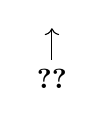
\begin{tikzpicture}
            \node[below] (A) at (0,0) {\Cref{lem:2.23}};
            \draw[->] (A) to (0, 0.4);
        \end{tikzpicture}
        }}{\leq} \abs{L:M}
    \end{equation*}
    We must have equality throughout, and so $\abs{L:M} = \abs{\Aut_M(L)} = \abs{H}$.
    Hence by \cref{thm:2.24} we have $M \leq L$ is a finite Galois extension and $H = \Gal(L/M)$.
\end{proof}
\begin{nthm}\label{thm:3.4}
    Let $K \leq L$ be a finite field extension. Then the following are equivalent:
    \begin{enumerate}[label=(\roman*)]
        \item $K \leq L$ is Galois
        \item $L^H = K$ when $H = \Aut_K(L)$
    \end{enumerate}
\end{nthm}

\begin{proof}
    \textbf{(i) $\Rightarrow$ (ii):} Let $M = L^H$ where $H = \Aut_K(L)$.
    By \nameref{thm:3.3}, $M \leq L$ is a Galois extension, and $\abs{L:M} = \abs{\Gal(L/M)}$ and $H = \Gal(L/M)$.

    However if $K \leq L$ is Galois then $\abs{H} = \abs{\Aut_K(L)} = \abs{L:K}$ by \cref{thm:2.24}.
    Thus $\abs{L:M} = \abs{L:K}$ and so $M = K$.

    \textbf{(ii) $\Leftarrow$ (i):} Use \cref{thm:3.3}.
\end{proof}
\begin{proof}[Proof of \nameref{thm:3.2}]
    \leavevmode
    \begin{enumerate}[label=(\roman*)]
        \item Composing the maps $H \to L^H$ and $M \to \Gal(L /M)$ gives $H \to H$ by \cref{thm:3.3}.
            Also $M \longrightarrow \Gal(L/M) \longrightarrow L^H$ where $H = \Gal(L/M)$ yields $M$ since $M \leq L^H$ where $H = \Gal(L/M)$ and
            \begin{equation*}
                \abs{L:L^H} \underset{\begin{subarray}{c}(\ref{thm:2.24})\\(\ref{thm:3.3})\end{subarray}}{=} \abs{H} = \abs{\Gal(L/M)} \underset{(\ref{thm:2.24})}{=} \abs{L:M}
            \end{equation*}
            So $M = L^H$.
        \item Take $H \leq \Gal(L/K)$, then $L^{\phi H \phi^{-1}} = \phi(L^H)$ when $\phi \in \Gal(L/K)$.
            So by (i), $H$ is normal iff $\phi(L^H) = L^H$. Set $M = L^H$.

            We'll show that $K \leq M$ is normal iff $\phi(M) = M \quad \forall \phi \in \Gal(L/K)$.
            $K \leq M$ is normal $\implies \phi(M) = M$ by remark 2 after the statement of \nameref{thm:3.2}.

            Conversely if $\phi(M) = M \quad \forall \phi \in \Gal(L/K)$, pick $\alpha \in M$ and let $f_\alpha(t)$ be its minimal polynomial over $K$.
            Take $\beta$ to be a root of $f_\alpha(t)$ in $L$ (possible by normality).
            Then there is a $K$-homomorphism
            \begin{equation*}
                \begin{tikzcd}[row sep=tiny, column sep=small]
                    K(\alpha) \cong \frac{K[t]}{(f_\alpha(t))} \ar[r] & K(\beta) \cong \frac{K[t]}{(f_\alpha(t))} \leq L \\
                    \alpha \ar[r, mapsto] & \beta.
                \end{tikzcd}
            \end{equation*}
            This extends to a $K$-homomorphism $\phi:L \to L$.

            However we are assuming $\phi(M) = M$ and so $\phi(\alpha) = \beta \in M$. Thus $K \leq M$ is normal.
            Note that $K \leq L^H$ is separable since $K \leq L^H \leq L$ and $K \leq L$ separable.

        \item By remark 2 after statement of \cref{thm:3.2}, the restriction map
            \begin{equation*}\theta:\Gal(L/K) \rightarrow \Gal(L^H/K)\end{equation*}
            is defined.
            Surjectivity follows from being able to extend a $K$-homomorphism $L^H \to L^H \leq L$ to a $K$-homomorphism $L \to L$ by \cref{cor:2.10}.
            Clearly $H \leq \Ker \theta$. However
            \begin{align*}
                \frac{\abs{L:K}}{\abs{\Ker \theta}} &= \frac{\Gal(L/K)}{\abs{\Ker \theta}} \\
                                                    &= \abs{\Gal(L^H/K)} \quad \text{by surjectivity of } \theta \\
                                                    &= \abs{L^H:K} \quad \text{since } K \leq L^H \text{ is Galois} \\
                                                    &= \frac{\abs{L:K}}{\abs{L:L^H}} \quad \text{by Tower law}
            \end{align*}
            So $\abs{\Ker \theta} = \abs{L:L^H} = \abs{\Gal(L/L^H)} = \abs{H}$ by \cref{thm:3.3}, so $H = \Ker \theta$. \qedhere
    \end{enumerate}
\end{proof}
\subsection{Galois groups of polynomials}

















\begin{nlemma}\label{lem:3.6}
    Suppose $f(t)$ is separable, $f(t) = g_1(t) \dotsm g_s(t)$ with $g_i(t)$ irreducible in $K[t]$ is a factorisation in $K[t]$.
    Then the orbits of $\Gal(f)$ on the roots of $f(t)$ correspond to the factors $g_j(t)$.
    \begin{equation*}
        \text{Two roots are in the same orbit} \iff \text{they are roots of the same } g_j(t).
    \end{equation*}
    In particular, if $f(t)$ is irreducible in $K[t]$ there is one orbit, i.e., $\Gal(f)$ acts transitively on the roots of $f(t)$.
\end{nlemma}
\begin{proof}
    Let $\alpha_k, \alpha_l$ be in the same orbit under $\Gal(f)$.
    Thus there is $\phi \in \Gal(f)$ with $\alpha_l = \phi(\alpha_k)$.
    But if $\alpha_k$ is a root of $g_j(t)$ then $\phi(\alpha_k) = \alpha_l$ is also a root of $g_j(t)$.

    Conversely, if $\alpha_k, \alpha_l$ are roots of $g_j(t)$ then
    \begin{equation*}
        \begin{tikzcd}
            K(\alpha_k) \rar[phantom,"\cong"] \ar[rr,bend right, "\phi_0"'] & \frac{K[t]}{(g_j(t))} \rar[phantom,"\cong"] & K(\alpha_l) \rar[phantom,"\leq"]& L
        \end{tikzcd}
    \end{equation*}
    with $\phi_0(\alpha_k) = \alpha_l$.
    $\phi_0$ extends to a $\phi:L \to L \in \Gal(L/K)$, thus $\alpha_k, \alpha_l$ are in the same orbit.
\end{proof}


\begin{nlemma}\label{lem:3.7}
    The transitive subgroups of $S_n$ for $n \leq 5$ are
    \begin{center}
        \begin{tabular}{rl}
            $n=2$:  & $S_2 \; (\cong C_2)$ \\
            $n=3$:  & $A_3 \; (\cong C_3), \; S_3$ \\
            $n=4$:  & $C_4, \; V_4, \; D_8, \; A_4, \; S_4$ \\
            $n=5$:  & $C_5, \; D_{10}, \; H_{20}, \; A_5, \; S_5$\\
        \end{tabular}
    \end{center}
    where $H_{20}$ is generated by a 5-cycle and a 4-cycle.
\end{nlemma}
\begin{proof}
    Exercise.
\end{proof}
\begin{nthm}\label{thm:3.8}
    Let $p$ be a prime, and $f(t)$ irreducible $\in \Q[t]$ of degree $p$.
    Suppose $f(t)$ has exactly 2 non-real roots in $\C$.
    Then $\Gal(f)$ over $\Q \cong S_p$.
\end{nthm}
\begin{proof}
    $\Gal(f)$ acts on the $p$ distinct roots of $f(t)$ in a splitting field $L$ of $f(t)$ (in $\C$).
    By \cref{lem:3.6}, the irreducibility of $f(t)$ implies that $\Gal(f)$ is acting transitively on the $p$ roots.
    By the orbit-stabiliser theorem, $p \mid \abs{\Gal(f)}$ but $\abs{\Gal(f)} \leq \abs{S_p} = p!$ and so $\Gal(f)$ has a Sylow $p$-subgroup of order $p$, necessarily cyclic.
    Thus, $\Gal(f)$ contains a $p$-cycle.

    The supposition that we have precisely 2 non-real roots gives that complex conjugation yields a transposition in $\Gal(f)$.
    The $p$-cycle and transposition generate the whole of $S_p$.
\end{proof}

\begin{proof}
    $f(t)$ is irreducible by \nameref{thm:1.16} with $p=3$.
    We want to show that $f(t)$ has three real roots, two non-real ones and apply \cref{thm:3.8}.
    \begin{equation*}
        f(-2) = -17, \; f(-1) = 8, \; f(1) = -2, \; f(2) = 23
    \end{equation*}
    and $f'(t) = 5t^4 - 6$ which has two real roots.
    From the intermediate value theorem, $f$ has at least three real roots, and by Rolle's theorem there are at most three real roots, so we are done.
\end{proof}


\begin{nlemma}\label{lem:3.11}
    Let $f(t)$ be separable $\in K[t]$ of degree $n$ with $\chara K \neq 2$.
    Then
    \begin{equation*}\Gal(f) \leq A_n \iff D(f)\text{ is a square in }K.\end{equation*}
\end{nlemma}
\begin{proof}
    Let $L$ be a splitting field of $f(t)$ over $K$.
    Then $D(f) \neq 0$ and is fixed by all elements of $G = \Gal(L/K)$ as the latter permutes the roots.
    Thus $D \in K$, since $L^G = K$ (by Galois correspondence).

    On the other hand, if $\sigma\in G$ then $\sigma(\Delta) = (\mathrm{sgn} \sigma) \Delta$ where we're regarding $G$ as a subgroup of $S_n$ and the signature of $\sigma$:
    \begin{equation*}
        \mathrm{sgn} \sigma =
        \begin{cases}
            +1 & \text{if $\sigma$ even} \\
            -1 & \text{if $\sigma$ odd}
        \end{cases}
    \end{equation*}
    (This is where we need $\chara K \neq 2$).

    Thus if $G \leq A_n$ we get that $\Delta$ is fixed by all $\sigma \in G$.
    Thus $\Delta \in K = L^G$.
    Otherwise if $G \nleq A_n$, we get $\sigma(A) = -\Delta$ if $\sigma$ is an odd permutation, and so $\Delta \notin K=L^G$.
    Note that if $D$ does have square roots, they must be $\pm \Delta$.
\end{proof}








\begin{nthm}[Mod $p$ reduction]\label{thm:3.13}
    Let $f(t) \in \Z[t]$ be monic of degree $n$ with $n$ distinct roots in a splitting field.
    Let $p$ be a prime such that $\overline{f}(t)$, the reduction of $f(t)$ mod $p$ also has $n$ distinct roots in a splitting field.
    Let $\overline{f}(t) = \overline{g_1}(t) \dotsm \overline{g_s}(t)$ be the factorisation into irreducibles in $\F_p[t]$ with $n_j = \deg \overline{g_j}(t)$.
    Then $\Gal(\overline{f}) \hookrightarrow \Gal(f)$ and has an element of cycle type $(n_1, n_2, \dotsc, n_s)$.
\end{nthm}
\begin{proof}
    We will talk about the last sentence after thinking about Galois groups of finite fields.
    The fact that $\Gal(\overline{f}) \hookrightarrow \Gal(f)$ is from Number Fields - see Tony Scholl's teaching page on Galois.
\end{proof}

\subsection{Galois Theory of Finite Fields}






















\begin{nthm}[Galois groups of finite fields]\label{thm:3.16}
    Let $\F$ be a finite field with $\abs{\F} = p^r$.
    Then $\F_p \leq \F$ is a Galois extension with $\Gal(\F/\F_p) = G$, a cyclic group with the Frobenius automorphism as generator.
\end{nthm}
\begin{proof}
    It remains to show that the order of the Frobenius automorphism is $r$.
    Suppose $\phi^s = \mathrm{id}$.
    Then $\alpha^{p^s} = \alpha \; \forall \alpha \in \F$.
    But $t^{p^s} - t$ has at most $p^s$ roots in $\F$, so we deduce that $s \geq r$.
    Observe that $\phi^r = \mathrm{id}$ since $\alpha^{p^n} = \alpha$, $\forall \alpha \in \F$.

    Now apply the \nameref{thm:3.2}:
    \begin{equation*}
        \{\F_p \leq M \leq \F \text{ intermediate fields } M\} \longleftrightarrow \{\text{subgroups } H \leq G\}
    \end{equation*}
    where $G = \Gal(\F/\F_p)$ is cyclic.

    But we know all about subgroups of a cyclic group with generator $\phi$ of order $r$.
    There is exactly one subgroup of order $s$ for each $s \mid r$ generated by $\phi^\frac{r}{s}$.
    The corresponding intermediate subfields are the fixed fields $\F^{\langle \phi^\frac{r}{s} \rangle}$, and $\abs{\F:\F^{\langle \phi^\frac{r}{s} \rangle}} = s$.
    By the Tower Law, $\abs{\F^{\langle \phi^\frac{r}{s} \rangle}:\F_p} = \frac{r}{s}$.
    Observe that all subgroups of cyclic groups are normal and therefore all our intermediate fields are normal extensions of $\F_p$.

    By \cref{thm:3.2} part (iii), $\Gal(\F^{\langle \phi^\frac{r}{s} \rangle}/F_p) \cong \Gal(\F/\F_p) / H$ where $H = \langle \phi^\frac{r}{s} \rangle$.
\end{proof}
\begin{ncor}\label{cor:3.17}
    Let $\F_p \leq M \leq \F$ be finite fields.
    Then $\Gal(\F/M)$ is cyclic, generated by $\phi^u$, where $\phi$ is the Frobenius automorphism and $\abs{M} = p^u$ and $M$ is the fixed field of $\langle \phi^u \rangle$.
\end{ncor}
\begin{proof}
    Set $n = \frac{r}{s}$.
\end{proof}
\begin{nthm}[Existence of finite fields]\index{finite field!existence}\label{thm:3.18}
    Let $p$ be a prime and $u \geq 1$.
    Then there is a field of order $p^u$, unique up to isomorphism.
\end{nthm}
\begin{proof}
    Consider the splitting field $L$ of $f(t) = t^{p^u} - t$ over $\F_p$.
    It is a finite Galois extension $\F_p \leq L$.
    However the roots of $f(t)$ form a field, the fixed field of $\phi^u$.
    Set $L = \F$ and $\abs{\F :\F_p} = u$.
\end{proof}

\clearpage
\section{Cyclotomic and Kummer extensions}
\subsection{Cyclotomic extensions}




























% can i change this to a lemma




\begin{nlemma}\label{lem:4.5}
    $\Phi_m(t) \in \Z[t]$ if $\chara K = 0$ (with $\Q \hookrightarrow K$, prime subfield).
    $\Phi_m(t) \in \F_p[t]$ if $\chara K = p$ (with $\F_p \hookrightarrow K$, prime subfield).
\end{nlemma}
\begin{proof}
    Induct on $m$. $m=1$ is clearly true.

    For $m>1$, consider
    \begin{equation*}
        f(t) = t^m - 1 = \Phi_m(t) \left(\prod_{\substack{d \mid m \\ d \neq m}} \Phi_d(t)\right).
    \end{equation*}
    Note that $\prod_{\substack{d \mid m \\ d \neq m}} \Phi_d(t)$ is monic and is defined in $\Z[t]$ or $\F_p[t]$ by induction.

    If $\chara K = 0$, we deduce $\Phi_m(t) \in \Q[t]$ by division of polynomials and by Gauss' Lemma it is in $\Z[t]$.
    If $\chara K = p > 0$, we deduce by division that $\Phi_m(t) \in \F_p[t]$.
\end{proof}
\begin{nlemma}\label{lem:4.6}
    The homomorphism $\theta: G \to (\Z/m\Z)^\times$ defined in \cref{def:4.3} is an isomorphism iff $\Phi_m(t)$ is irreducible.
\end{nlemma}
\begin{proof}
    We know from \cref{lem:3.6} that the orbits of $G = \Gal(L/K)$ correspond to the factorisation of $f(t)$ in $K[t]$.
    In particular, the primitive $m$th roots of unity form one orbit iff $\Phi_m(t)$ is irreducible.
    Then $\theta$ is surjective iff $\Phi_m(t)$ is irreducible.
\end{proof}
\begin{nthm}\label{thm:4.7}
    Let $L$ be the $m$th cyclotomic extension of finite field $\F = \F_q$ where $q = p^n$.
    Then the Galois group $G = \Gal(L/\F)$ is isomorphic to the cyclic subgroup of $(\Z/m\Z)^\times$ generated by $q$.
\end{nthm}
\begin{proof}
    We know from \cref{cor:3.17} that $G$ is generated by $\alpha \mapsto \alpha^{p^n} = \alpha^q$ so $\theta(G) = \langle q\rangle \leq (\Z/m\Z)^\times$.
\end{proof}



\begin{nthm}\label{thm:4.8}
    For all $m > 0$, $\Phi_m(t)$ is irreducible in $\Z[t]$ and hence in $\Q[t]$.
    Thus $\theta$ in \cref{def:4.3} is an isomorphism and thus $\Gal(\Q(\xi)/\Q) \cong (\Z/m\Z)^\times$ where $\xi =$ primitive $m$th root of unity.
\end{nthm}

\begin{proof}[Proof of \cref{thm:4.8}]
    Gauss' Lemma gives us that irreducibility in $\Z[t]$ implies irreducibility in $\Q[t]$.
    From \cref{lem:4.5}, irreducibility corresponds to surjectivity of $\theta$.
    It's left to show that $\Phi_m(t)$ is irreducible in $\Z[t]$.

    Suppose not, and $\Phi_m(t) = g(t) h(t)$ in $\Z[t]$ with $g(t)$ irreducible. monic and $\deg g(t) \lneqq \deg \Phi_m(t)$.
    Let $\Q \leq L$ be the $m$th cyclotomic extension and $\xi$ be a root of $g(t)$, $\xi$ primitive $m$th root of unity.

    \textbf{Claim}: if $p \nmid m$, $p$ prime, then $\xi^p$ is also a root of $g(t)$ in $L$.
    Suppose not. Then $\xi^p$ is also a primitive $m$th root of 1, since $p \nmid m$, as a root of $\Phi_m(t)$.
    By the supposition, $\xi^p$ is a root of $h(t)$.
    Define $r(t) = h(t^p)$. Then $r(\xi) = 0$ but $g(t)$ is the minimal polynomial of $\xi$ over $\Q$.
    So $g(t) \mid r(t)$ in $\Q[t]$.

    By Gauss' Lemma, $r(t) = g(t) s(t)$ with $s(t) \in \Z[t]$.
    Now reduce mod $p$. $\overline{r}(t) = \overline{g}(t) \overline{s}(t)$.
    But $\overline{r}(t) = \overline{h}(t^p) = (\overline{h}(t))^p$.
    If $\overline{a}(t)$ is any irreducible factor of $\overline{g}(t)$ in $\F_p[t]$ then $\overline{a}(t) \mid (\overline{h}(t))^p$ and so $\overline{a}(t) \mid \overline{h}(t)$.
    But then $(\overline{a}(t))^2 \mid \overline{g}(t) \overline{h}(t) = \overline{\Phi_m}(t)$.
    Hence $\overline{\Phi_m}(t)$ has a repeated root and thus $t^m-1$ has repeated root mod $p$.
    Contradiction, since $p \nmid m$, so claim is true.

    Now consider a root $\gamma$ of $h(t)$.
    Then it is also a primitive root of 1 and so $\gamma = \xi^i$ for some $i$ with $(i, m) = 1$.
    Write $i = p_1 \dotsm p_k$ factorisation with $p_j$ prime, not necessarily distinct, $p_j \nmid m$.
    Applying the claim repeatedly we get that $\gamma$ is a root of $g(t)$, and so $\Phi_m(t)$ has a repeated root.

    Hence $\Phi_m(t)$ is irreducible over $\Q$.
\end{proof}


\subsection{Kummer Theory}






\begin{nthm}\label{thm:4.10}
    Let $f(t) = t^m - \lambda \in K[t]$ and $\chara K \nmid m$.
    Then the splitting field $L$ of $f(t)$ over $K$ contains a primitive $m$th root of unity $\xi$ and $\Gal(L/K(\xi))$ is cyclic of order dividing $m$.
    Moreover $f(t)$ is irreducible over $K(\xi)$ iff $\abs{L:K(\xi)} = m$.
\end{nthm}

\begin{proof}[Proof of \cref{thm:4.10}]
    Since $t^m - \lambda$ and $m t^{m-1}$ are coprime, we know that $t^m - \lambda$ has distinct roots $\alpha_1, \dotsc, \alpha_m$ in the splitting field $L$.
    Since $(\alpha_i \alpha_j^{-1})^m = \lambda \lambda^{-1} = 1$, the elements $1 = \alpha_1 \alpha_1^{-1}, \alpha_2 \alpha_1^{-1}, \dotsc, \alpha_m \alpha_1^{-1}$ are $m$ distinct $m$th roots of unity in $L$ and so
    \begin{equation*}
        t^m - \lambda = (t-\beta)(t-\xi\beta)(t-\xi^2 \beta)\dotsm (t-\xi^{m-1}\beta) \in L[t]
    \end{equation*}
    where $\beta = \alpha_1$ and $\xi$ primitive $m$th root of unity.

    So $L = K(\xi, \beta)$. Let $\sigma \in \Gal(L/K(\xi))$, which is determined by its action on $\beta$.
    Note that $\sigma(\beta)$ is another root of $t^m - \lambda$ and so $\sigma(\beta) = \xi^{j(\sigma)} \beta$, where $0 \leq j(\sigma) < m$.
    Also, if $\sigma, \tau \in \Gal(L/K(\xi))$ then
    \begin{equation*}
        \tau\sigma(\beta) = \tau(\xi^{j(\sigma)} \beta) = \xi^{j(\sigma)} \tau(\beta) = \xi^{j(\sigma)} \xi^{j(\tau)} \beta
    \end{equation*}
    since $\xi$ is fixed by $\tau$.
    Thus $\sigma \to j(\sigma)$ gives a group homomorphism
    \begin{equation*}
        \theta:\Gal(L/K(\xi)) \to \Z/m\Z.
    \end{equation*}

    Note that $j(\sigma) = 1$, only if $\sigma$ is the identity and so $\theta$ is injective.
    Hence $\Gal(L/K(\xi)) \cong $ subgroup of $\Z/m\Z$.
    Finally $\abs{L:K(\xi)} = \abs{\Gal(L/K(\xi))} \leq m$ with equality exactly when the action of $\Gal(L/K(\xi))$ is transitive on the roots, i.e.\ when $t^m-1$ is irreducible over $K(\xi)$ by \cref{lem:3.6}.
\end{proof}

% \begin{eg}
%     Take $f(t) = t^5 - 2$ over $\mathbb{Q}$, irreducible by \nameref{thm:1.16}, and $L$ the splitting field of $f(t)$ over $\mathbb{Q}$.
%     Let $\xi$ be a \hyperlink{def:primRoot}{primitive fifth root of unity}.
% \end{eg}


\begin{nthm}\label{thm:4.11}
    Suppose $K \leq M$ is a cyclic extension with $\abs{L:K} = m$, where $\chara K \nmid m$ and that $K$ contains a primitive $m$th root of unity.
    Then $\exists \lambda \in K$ such that $t^m - \lambda$ is irreducible over $K$ and $K$ is the splitting field of $t^m - \lambda$ over $K$.
    If $\beta$ is a root of $t^m - \lambda$ in $L$, then $L = K(\beta)$.
\end{nthm}


\begin{nlemma}\label{lem:4.13}
    Let $\phi_1, \dotsc, \phi_n$ be embeddings of a field $K$ into a field $L$.
    Then there do not exist $\lambda_1, \dotsc, \lambda_n$ not all zero such that $\lambda_1 \phi_1(x) + \dotsb + \lambda_n \phi_n(x) = 0 \; \forall x \in K$.
\end{nlemma}
\begin{proof}
    Example sheet 2, question 10.
\end{proof}
\begin{proof}[Proof of \cref{thm:4.11}]
    Let $\Gal(L/K) = \langle \sigma \rangle$ of order $m$.
    Observe that $1, \sigma, \sigma^2, \dotsc, \sigma^{m-1}$ are distinct maps $L \to L$, and we can apply \cref{lem:4.13}.
    There exists $\alpha \in L$ such that
    \begin{equation*}
        \beta = \alpha + \xi \sigma(\alpha) + \dotsb + \xi^{m-1} \sigma^{m-1}(\alpha) \neq 0
    \end{equation*}
    where $\xi$ is a primitive $m$th root of unity.
    Observe that $\sigma(\beta) = \xi^{-1} \beta \neq \beta$ and so $\beta \notin K$, the fixed field of $\Gal(L/K)$.

    $\sigma(\beta^m) = (\sigma(\beta))^m = \beta^m$. Let $\lambda = \beta^m \in K$.
    But $t^m - \lambda = (t-\beta)(t-\xi\beta)\dotsm(t-\xi^{m-1}\beta)$ in $L[t]$, and so $K(\beta)$ is the splitting field of $t^m - \lambda$ over $K$ (recall $\xi \in K$).
    Observe that $1, \sigma, \dotsc, \sigma^{m-1}$ are distinct $K$-automorphisms of $K(\beta)$ and so $\abs{K(\beta):K)} \geq m$.

    So $L = K(\beta) = K(\xi\beta)$ since $\xi \in K$.
    $t^m - \lambda$ is the minimal polynomial of $\beta$ over $K$ and hence is irreducible.
\end{proof}

% lecture 18
\subsection{Cubics}

































{
}





























\subsection{Quartics}







































% Lecture 19
























\subsection{Solubility by radicals}





















\begin{nlemma}\label{lem:4.16}
    A finite group $G$ is soluble if and only if we have
    \begin{equation*}
        \{e\} = G_m \lhd G_{m-1} \lhd \dotsb \lhd G_1 \lhd G_0 = G
    \end{equation*}
    with $G_i/G_{i+1}$ cyclic.
\end{nlemma}
\begin{proof}
    $(\Leftarrow)$ is immediate.
    $(\Rightarrow)$. We know about the structure of finite abelian groups.
    If $A$ abelian then there is a chain
    \begin{equation*}
        \{e\} = A_r \lhd A_{r-1} \lhd \dotsb \lhd A_0 = A
    \end{equation*}
    with $A_r / A_{r+1}$ cyclic.
    Thus if we have a chain with abelian factors $G_i/G_{i+1}$ we can refine it to have cyclic factors.
\end{proof}

\begin{nlemma}\label{lem:4.18}
    Let $K \lhd G$. Then $G/K$ abelian $\iff G' \leq K$.
\end{nlemma}
\begin{proof}
    \begin{align*}
        G/K \text{ abelian} &\iff Kg_1 Kg_2 Kg_1^{-1} K g_2^{-1} = K \quad \forall g_1, g_2 \in G\\
                            &\iff g_1 g_2 g_1^{-1} g_2^{-1} \in K \\
                            &\iff G' \leq K. \qedhere
    \end{align*}\qedhere
\end{proof}


\begin{nlemma}\label{lem:4.20}
    For $G$ finite, $G$ is soluble $\iff G^{(m)} = \{e\}$ for some $m$.
\end{nlemma}
\begin{proof}
    If $G^{(m)} = \{e\}$ then the derived series gives a chain in the definition of solubility.

    Conversely if there is such a chain
    \begin{equation*}
        G \rhd G_1 \rhd G_2 \rhd \dotsb \rhd G_m = \{e\}
    \end{equation*}
    with $G_i/G_{i+1}$ abelian then an easy induction shows that $G^{(j)} \leq G_j$ and so $G^{(m)} = \{e\}$.
\end{proof}
\begin{nlemma}\label{lem:4.21}\leavevmode
    \begin{enumerate}[label=(\roman*)]
        \item Let $H \leq G$, $G$ soluble. Then $H$ soluble.
        \item Let $H \lhd G$, then $G$ soluble $\iff H$ and $G/H$ both soluble.
    \end{enumerate}
\end{nlemma}
\begin{proof}\leavevmode
    \begin{enumerate}[label=(\roman*)]
        \item $G$ soluble $\implies G^{(m)} = \{e\}$ by \cref{lem:4.20}.
            But $H^{(m)} \leq G^{(m)}$ and so $H$ soluble by \cref{lem:4.20}.
        \item Let $H \lhd G$, then $G$ soluble $\implies H$ soluble by (i).
            $G$ soluble $\implies G^{(m)} = \{e\}$, say.
            Observe that
            \begin{equation*}\left(\frac{G}{H}\right)' = \frac{G'H}{H} \leq \frac{G}{H}.\end{equation*}
            Similarly,
            \begin{equation*}
                (\frac{G}{H})^{(j)} = \frac{G^{(j)}H}{H} \leq \frac{G}{H}.
            \end{equation*}
            Thus $(G/H)^{(m)} = H/H$, a trivial subgroup of $G/H$ and so $G/H$ soluble.

            Now consider the converse. Suppose that $H$ and $G/H$ are soluble.
            $H^({r}) = \{e\}$ and $(G/H)^{(s)} = H/H$.
            But
            \begin{equation*}
                \left(\frac{G}{H}\right)^{(s)} = \frac{G^{(s)}H}{H}
            \end{equation*}
            so $G^{(s)}H = H$ thus $G^{(s)} \leq H$. Hence $G^{(r+s)} \leq H^{(r)} = \{e\}$.
            Thus $G$ is soluble by \cref{lem:4.20}.
    \end{enumerate}
\end{proof}

\begin{nthm}\label{thm:4.22}
    Let $K$ be a field and $f(t) \in K[t]$.
    Assume $\chara K= 0$. Then $f(t)$ is soluble by radicals over $K \iff \Gal f$ over $K$ is soluble.
\end{nthm}

\begin{ncor}\label{cor:4.23}
    If $f(t)$ is a monic irreducible polynomial $\in K[t]$ with $\Gal(f) \cong A_5$ or $S_5$ then $f(t)$ is not soluble by radicals (with $\chara K$ = 0).
\end{ncor}

\begin{nlemma}\label{lem:4.24}
    If $K \leq N$ is an extension by radicals then $\exists N'$ with $N \leq N'$ with $K \leq N'$ is an extension by radicals, with $K \leq N'$ a Galois extension.
\end{nlemma}
\begin{proof}[Proof of \cref{thm:4.22}]
    Suppose $f(t)$ is soluble by radicals.
    Thus if $L$ is the splitting field of $f(t)$ over $K$ then $L$ lies in an extension of $K$ by radicals
    \begin{equation*}
        K = L_0 \leq L_1 \leq \dotsb \leq L_m
    \end{equation*}
    with each $L_i \leq L_{i+1}$ cyclotomic or Kummer.

    With \cref{lem:4.24}, we may assume $L_m$ is Galois over $K$.
    By \nameref{thm:3.2} there is a corresponding chain of subgroups of $\Gal(L_m/K)$.
    Our previous discussion at the beginning of this section (before \cref{lem:4.13}) we know that $\Gal(L_m/K)$ is soluble.

    But $F \leq L \leq L_m$ with $K \leq L$ Galois.
    By the \nameref*{thm:3.2}, $\Gal(L/K) \cong \Gal(L_m/K)/\Gal(L_m/L)$.

    But quotients of soluble groups are soluble, so $\Gal(L/K)$ is soluble.
\end{proof}
\begin{proof}[Proof of \cref{lem:4.24}]
    We have $K = L_0 \leq L_1 \leq \dotsb \leq L_m$ with each $L_i \leq L_{i+1}$ cyclotomic or Kummer,
    and we want to embed this into a Galois extension of the same form.

    Assume $\chara K = 0$. By the \nameref{thm:2.17}, $L_m = K(\alpha_1)$ for some $\alpha_1$.
    Let $g(t)$ be the minimal polynomial of $\alpha_1$ over $K$ with splitting field $M$.
    Thus $M = K(\alpha_1,\alpha_2,\dotsc,\alpha_n)$ where $\alpha_1, \dotsc, \alpha_n$ are roots of $g(t)$.

    There are $K$-homomorphisms
    \begin{align*}
        \phi_i : M &\longrightarrow M \\
        \alpha_1 &\longmapsto \alpha_i
    \end{align*}
    extending the $K$-homs $K(\alpha_1) \to K(\alpha_i) \leq M$.

    The tower $K \leq \phi_i(K) \leq \phi_i(L_1) \leq \dotsb \leq \phi_i(L_m) = K(\alpha_i)$ with cyclotomic or Kummer extensions as before,
    Consider $L_m = K(\alpha_1) \leq \phi_2(L_1)(\alpha_1) \leq \phi_2(L_2)(\alpha_1) \leq \dotsb \leq \phi_2(L_m)(\alpha_1) = K(\alpha_1,\alpha_2)$.

    Consider the extension $\phi_2(L_j)(\alpha_1) \leq \phi_2(L_{j+1})(\alpha_1)$:
    \begin{enumerate}[label={}]
        \item \textbf{if $L_j \leq L_{j+1}$ is cyclotomic} then all the roots of unity adjoined are now in $L_m = K(\alpha_1)$ and so $\phi_2(L_j)(\alpha_1) = \phi_2(L_{j+1})(\alpha_1)$.
        \item \textbf{if $L_j \leq L_{j+1}$ is Kummer} then we obtain $L_{j+1}$ by adjoining roots of an element of $L_j$ and so we obtain $\phi_2(L_{j+1})$ by adjoining roots of an element in $\phi_2(L_j)$.
            Hence we get from $\phi_2(L_j)(\alpha_1)$ to $\phi_2(L_{j+1})(\alpha_1)$ by adjoining roots of an element of $\phi_2(L_j)$. So it's a Kummer extension.
    \end{enumerate}

    Now continue to get suitable chain $K(\alpha_1,\alpha_2) \leq \dotsb \leq K(\alpha_1, \alpha_2, \alpha_3)$.

    Thus we get a suitable chain from $K$ to $K(\alpha_1, \dotsc, \alpha_n) = M$.
    Observe that $K \leq M$ is Galois.
\end{proof}
\begin{proof}[Converse of \Cref{thm:4.22}]
    Suppose $G = \Gal(f)$ over $K$ is soluble (and $\chara K=0$).
    Let $L$ be the splitting field of $f(t)$ over $K$ and so $|G| = |L:K| = n$.
    Set $m = n!$ and let $\xi$ be a primitive root of unity and consider $L(\xi)$.
    \begin{center}
        \begin{tikzpicture}[node distance=2cm]
            \node (v) at (0,0) {};
            \node (Lx) [above of=v] {$L(\xi)$};
            \node (Kx) [left of=v]  {$K(\xi)$};
            \node (L)  [right of=v] {$L$};
            \node (K)  [below of=v] {$K$};
            \draw (Lx) -- (Kx) node[midway,anchor=south east]{$\leq n$} -- (K) -- (L) node[midway,anchor=north west]{$n$} -- (Lx);
        \end{tikzpicture}
    \end{center}
    Our proof is similar to that used for cubics.
    Observe that $|L(\xi):K(\xi)| \leq n$. By the \nameref{thm:2.17} $L=K(\alpha)$ for some $\alpha$ with minimal polynomial $g(t)$ say of degree $n$.
    Then $L(\xi) = K(\xi)(\alpha)$ and the minimal polynomial of $\alpha$ over $K(\xi)$ divides $g(t)$ and so is of degree $\leq n$.

    Then $\Gal(L(\xi)/K)$ is soluble since $\Gal(L(\xi)/L)$ is soluble and $\Gal(L/K) \cong \frac{\Gal(L(\xi)/K)}{\Gal(L(\xi)/L)}$ soluble by \nameref{thm:3.2} and \Cref{lem:4.21}.
    Then the subgroup $\Gal(L(\xi)/K(\xi)) \leq \Gal(L(\xi)/K)$ is soluble by \Cref{lem:4.21}.

    Thus there is a chain of subgroups
    \begin{equation*}
        \Gal(L(\xi)/K(\xi)) = G_0 \rhd G_1 \rhd \dotsb \rhd G_m = \{e\},
    \end{equation*}
    with $G_i/G_{i+1}$ cyclic (using \Cref{lem:4.16}).

    Now use the \nameref{thm:3.2} to get a corresponding chain of fields $K(\xi) \leq K_1 \leq \dotsb \leq K_m = L(\xi)$, with each $K_i \leq K_{i+1}$ Galois, with cyclic Galois group.
    By \Cref{thm:4.11}, all these extensions are Kummer (not all the extensions are of degree $\leq n$ and so we have the appropriate roots of unity).
    Thus we've embedded $L$ in an extension of $K$ by radicals.
\end{proof}

\clearpage
\section{Final Thoughts}
\subsection{Algebraic closure}



\begin{nlemma}\label{lem:5.3}
    If $K \leq L$ is algebraic and every polynomial in $K[t]$ splits completely over $L$, then $L$ is an algebraic closure of $K$.
\end{nlemma}
\begin{proof}
    We need to show $L$ is algebraically closed.
    Suppose $L \leq L(\alpha)$ is a finite extension, and $f_\alpha(t) = t^n + a_{n-1} t^{n-1} + \dotsb + a_0$ is the minimal polynomial of $\alpha$ over $L$.
    Let $M = K(a_0, a_1, \dotsc, a_{n-1})$.
    Then $M \leq M(\alpha)$ is a finite extension.
    But each $a_i$ is algebraic over $K$ and so $|M:K|<\infty$.
    Hence $|M(\alpha):K| < \infty$ by \nameref{thm:towerLaw} and so $\alpha$ is algebraic over $K$.
    The minimal polynomial over $K$ must split over $L$, and so $\alpha \in L$.
    Thus any algebraic extension of $L$ is $L$ itself.
\end{proof}


\begin{nlemma}[Zorn's Lemma]\index{Zorn's lemma}\label{lem:zorn}
    Let $(\mathcal{S},\leq)$ be a non-empty partially ordered set.
    Suppose that any chain has an upper bound in $\mathcal{S}$.
    Then $\mathcal{S}$ has a maximal element.
\end{nlemma}
\begin{nlemma}\label{lem:5.6}
    Let $R$ be a ring. Then $R$ has a maximal ideal.
\end{nlemma}
\begin{proof}
    Let $\mathcal{S}$ be the set of proper ideals of $R$.
    This is is non-empty, since $(0)$ is proper.
    Partially order $\mathcal{S}$ by inclusion.
    Any ideal $I$ is proper $\Longleftrightarrow 1 \notin I$.
    Any chain of proper ideals has an upper bound in $\mathcal{S}$, namely the union of the chain.
    \nameref{lem:zorn} gives that $\mathcal{S}$ has a maximal element, i.e.\ a maximal ideal of $R$.
\end{proof}
\begin{nthm}[Existence of algebraic closures]\index{algebraic closure!existence}\label{thm:5.7}
    For any field $K$ there is an algebraic closure.
\end{nthm}
\begin{proof}
    Let
    \begin{equation*}
        \mathcal{S} = \set{(f(t),j) | f(t) \text{ irreducible, monic in } K[t], 1 \leq j \leq \deg f}
    \end{equation*}
    For each pair $s = (f(t),j) \in \mathcal{S}$ we introduce an indeterminate $X_s = X_{f,j}$.
    Consider the polynomial ring $K[X_s: s \in \mathcal{S}]$ and set
    \begin{equation*}\tilde{f}(t) = f(t) - \prod_{j=1}^{\deg g} (t - X_{f,j}) \in K[X_s: s \in \mathcal{S}][t].\end{equation*}

    Let $I \lhd K[X_s : s \in \mathcal{S}]$ generated by all the coefficients of all the $\tilde{f}(t)$.
    Denote the coefficents of $\tilde{f}(t)$ by $a_{f,l}$ for $0 \leq l \leq \deg f$.

    Claim: $I \neq K[X_s : s \in \mathcal{S}]$.
    Proof: Suppose $1 \in I$ and aim for a contradiction.
    \begin{equation*}
        b_1 a_{f_1,l_1} + \dotsb + b_N a_{f_N,l_N} = 1 \quad \text{in } K[X_s : s \in \mathcal{S}]. \tag{$+$} \label{eq:plus}
    \end{equation*}
    Let $L$ be a splitting field for $f_1(t) \dotsm f_N(t)$.

    For each $i$, $f_i$ splits over $L$. $f_i(t) = \prod_{j=1}^{\deg f_i} (t-a_{ij})$.
    Define a $K$-linear ring homomorphism, identity on $K$,
    \begin{equation*}
        \begin{tikzcd}[row sep=tiny]
            \theta: K[X_s : s \in \mathcal{S}] \rar & L \\
            X_{f_i,j} \rar[maps to] & \alpha_{ij} \\
            X_s \rar[maps to] & 0 & \text{otherwise}.
        \end{tikzcd}
    \end{equation*}
    This induces a map $K[X_s : s \in \mathcal{S}] \to L[t]$.
    Then
    \begin{align*}
        \theta(\tilde{f}_i(t)) &= \theta(f_i(t)) - \prod_{j=1}^{\deg f_i} \theta(t - X_{f_i,j}) \\
                               &= f_i(t) - \prod_{j=1}^{\deg f_i} (t - \alpha_{i,j}) = 0.
    \end{align*}
    But then $\theta(a_{f_i,j}) = 0$ since $a_{f_i,j}$ are the coefficients of $\tilde{f_i}(t)$.
    But applying $\theta$ to \eqref{eq:plus} we get $0=1$.

    Then $I$ is a proper ideal of $K[X_s : s \in \mathcal{S}]$. By \nameref{lem:zorn} there is a maximal ideal $P$ of $K[X_s : s \in \mathcal{S}]$ containing $I$.
    Set $L_1 = K[X_s : s \in \mathcal{S}]/P$, a field.
    Thus we have a field extension $K \leq L_1$.

    Claim: $L_1$ is an algebraic closure of $K$.
    First show $K \leq L_1$ is algebraic: $L_1$ is generated by the maps $x_{f,j}$ of the $X_{f,j}$.
    However $\tilde{f}(t)$ has coefficients in $I$ and so its image $L_1[t]$ is the zero polynomial.
    Thus in $L_1[t]$,
    \begin{equation*}
        f(t) = \prod (t - x_{f,j}) \label{eq:23star}\tag{$*$}
    \end{equation*}
    and so $f(x_{f,j}) = 0$. Thus the $x_{f,j}$ are algebraic.

    Any element of $L_1$ involves only finitely many of the $x_{i,j}$ and so is algebraic over $K$.
    Moreover from \eqref{eq:23star} any $f(t) \in K[t]$ splits completely over $L_1$.

    The result follows from \Cref{lem:5.3}.
\end{proof}
\begin{nthm}\label{thm:5.8}
    Suppose $\theta: K \to L$ is a ring homomorphism and $L$ is algebraically closed.
    Suppose $K \leq M$ is an algebraic extension.
    Then $\theta$ can be extended to a homomorphism $\theta: M \to L$ (i.e.\ $\phi|_K = \theta$).
\end{nthm}
\begin{proof}
    Let
    \begin{equation*}
        \xi = \set{(N, \phi) | K \leq N \leq M, \phi \text{ a homomorphism } N \to L \text{ extending } \theta}.
    \end{equation*}
    Partially order $\xi$ with $(N_1, \phi_1) \leq (N_2, \phi_2)$ if $N_1 \leq N_2$ and $\phi_2|_{N_2} = \phi_1$.
    $\xi$ is non-empty since $(K, \theta) \in \xi$.

    If there is a chain $(N_1, \phi_1) \leq \dotsb$
    then set $N = \bigcup N_\lambda$. This is a subfield of $M$, and we can define $\psi: N \to L$ as follows:
    if $\alpha \in N$ then $\alpha \in N_\lambda$ for some $\lambda$ and we set $\psi(\alpha) = \phi_\lambda(\alpha)$. This is well defined.

    Then $(N,\psi)$ is an upper bound for our chain $\xi$.

    \nameref{lem:zorn} applies and gives a maximal element of $\xi$, $(N, \phi)$.
    We now show $N=M$.
    Given $\alpha \in M$, it is algebraic over $K$, and hence over $N$.
    Let $f_\alpha(t)$ be its minimal polynomial over $N$.
    But $\phi f(t)$ is in $L[t]$ and so splits completely over $L$, since $L$ is algebraically closed.

    So $\phi f(t) = (t-\beta_1)\dotsm(t-\beta_r)$, say.
    Since $\phi f(B_\gamma) = 0$ then there is a map
    \begin{equation*}
        \begin{tikzcd}
            N(\alpha) \cong \frac{N[t]}{(f\alpha(t))} \rar & L \\
            \alpha \rar[maps to] & \beta_1 & \text{extending} \phi
        \end{tikzcd}
    \end{equation*}
    Maximality of $(N,\phi)$ implies that $N(\alpha) = N$. So $\alpha \in N$, so $N = M$.
\end{proof}
\begin{nthm}[Uniquness of algebraic closures]\index{algebraic closure!uniqueness}\label{thm:5.9}
    If $K \leq L_1$, $L \leq L_2$ are two algebraic closures of $K$ then there exists an isomorphism $\phi:L_1 \to L_2$.
\end{nthm}
\begin{proof}
    By \Cref{thm:5.8} there is a homomorphism $\phi:L_1 \to L_2$ extending the embedding of $K$ into $L_2$.
    Since $K \leq L_2$ is algebraic, so too is $\phi(L_1)$. But $L_1$ is algebraically closed and so $\phi(L_1)$ is algebraically closed.
    So $L_2 = \phi(L_1)$ and $\phi$ is an isomorphism.
\end{proof}
\subsection{Symmetric polynomials and invariant theory}


















\begin{nthm}\label{thm:5.11}
    The fixed field $M = L^{s_n} = K(s_1, \dotsc, s_n)$ and the $s_1, \dotsc, s_n$ are algebraically independent over $K$ (in $L$).
\end{nthm}


\end{document}